\documentclass{uulm-assignment}
\usepackage{import}
\usepackage{tabularx}
\usepackage{listings}
\usepackage{hyperref}
\usepackage{CJKutf8}
\usepackage{graphicx}
\usepackage{float}

\setboolean{showsolutions}{false}

\ifthenelse{\boolean{showsolutions}}{
    \newcommand\mitloesung{1}%
}{
    \newcommand\mitloesung{0}%
}

\hypersetup{colorlinks=false,urlcolor=uulm-in}

\faculty{Institut für Softwaretechnik und Programmiersprachen\hspace{0.05cm}}
\course{Softwaregrundprojekt}
\semester{\hspace{0.05cm} WiSe 2022/23}
\supervisor{\hspace{7.9cm} Prof. Dr. Thomas Thüm, Sabrina Böhm, Valentin Kolb, Pascal Schiessle}


\assignmenttype{}
\assignmentno{}
\title{Pflichtenheft - Battle of the Centerländ (Team 08)}
\author{Team 08}

\newcommand{\game}{Battle of the Centerländ}

\begin{document}



    \maketitle
    
    
    
    \tableofcontents
    
    \newpage
    

    \section{Allgemeine Einleitung}

    \subsection{Einleitung}
     Das Entwickeln des rundenbasierten Taktik-Spiels „Battle of the Centerländ - ein Code sie alle zu knechten“ ist das Ziel des Softwaregrundprojekts. Das Spiel soll ein Multiplayer Spiel darstellen.\

In dem Spiel können zwei bis sechs Spielende im fiktiven Mittelerde im Jahr 3018 darum kämpfen, den Ring des dunklen Herren Saurons zu vernichten, um dessen Herrschaft ein Ende zu setzen. Damit sie dies durchführen können, müssen die Gefährten und weitere Abenteurer zum Schicksalsberg gelangen. Auf dem Weg warten jedoch viele Gefahren auf die Spielenden, die es zu bewältigen gibt. Dazu kommt, dass niemand der Spieler die jeweils anderen zuerst zum Ziel gelangen lassen möchte, wodurch die Mitspielenden also ebenso eine Herausforderung darstellen.
    
    \subsection{Motivation}
    Das Projekt soll uns auf spätere große Programmierprojekte vorbereiten. Es soll uns veranschaulichen wie man in Teams arbeitet und auch mit Code von anderen Gruppen Kompatibilität herstellt. Wir lernen dabei unsere Position in einem Team richtig einzuschätzen, also unsere Stärken und Schwächen verglichen mit den anderen Teammitgliedern für ein großes funktionierendes Team einzusetzen. Nicht zu vernachlässigen ist, dass durch solch ein Projekt auch unsere Fähigkeit der Kommunikation sowie Planung und Aufgabenverteilung innerhalb eines Teams gefördert wird.
Eine auftraggebende Person erhält hierbei einen Überblick über die oben genannten Fähigkeiten und kann unsere Teamleistung besser beurteilen und erhält zusätzlich ein amüsantes Spiel gegen Langeweile.
    \subsection{Vision}
    Da fertige Spiel soll ein rundenbasiertes Multiplayer-Strategiespiel darstellen. Das Spiel spielt in Centerländ einer fiktiven Welt angelehnt an Mittelerde aus den Herr der Ringe Romanen.
Ähnlich zu den Romanen handelt das Spiel davon, dass die Gefährten aufbrechen um den Ring des dunklen Herren Saurons im Schicksalsberg zu vernichten und somit dessen Herrschaft zu beenden. Im Gegensatz zu den Romanen ist es im Spiel das Ziel aber vor den anderen Charakteren am Berg anzukommen. \\

Das Spiel soll folgendermaßen ablaufen. Zu Spielbeginn kann jeder Spieler aus zwei zufällig vorgeschlagenen Charakteren einen auswählen. Diese haben keine speziellen Fähigkeiten und dienen ausschließlich zu visuellen Repräsentation im Spiel. Außerdem erhält jeder Spieler ein Kartenset samt den neun Handkarten. Zufällig werden den Spielenden ebenfalls noch Startfelder zugewiesen. Damit kann die erste Runde beginnen.\\
Eine Runde wird in zwei Phasen aufgeteilt. In der ersten Phase loggt jeder Spielende fünf seiner Handkarten ein. Die zweite Phase besteht nun aus den Zügen. Hierbei spielen alle Spieler ihre erste eingeloggte Karte. Hat jeder Spieler seine Karte gespielt werden vom Server alle auszuführenden Aktionen abgehandelt. Damit endet die erste Zugrunde und die zweite Phase wird mit den zweiten, dritten, vierten und fünften Karten jeweils wiederholt. 
Die Wahl der fünf Karten sowie deren Reihenfolge ist nun also entscheidend für den Spielverlauf und stellt den Strategischen Teil des Spiels dar. Damit das Spiel auch zur Unterhaltung von Einzelpersonen gespielt werden kann werden in diesem Fall diese Entscheidungen von einer KI getroffen.
Damit ist das Spiel in zwei Szenarien spielbar. Einmal als Multiplayer-Spiel über eine Netzwerkverbindung gegen Freunde und zum anderen auch zum alleinigen Gebrauch gegen eine KI.
    \subsection{Projektkontext}
    Der Kontext für das Projekt an der Universität Ulm im Kurs Softwareentwicklung ist der Aufbau eines Multiplayer-Spiels. 
Die Studierenden sind die primären Stakeholder des Projekts, da sie diejenigen sind, die das Multiplayer-Spiel entwickeln und implementieren werden. Sie werden von den Dozenten des Kurses begleitet, die als sekundäre Stakeholder fungieren und sich um die Organisation und Betreuung des Projekts kümmern.

Weitere Stakeholder könnten auch Personen sein, die das Multiplayer-Spiel später nutzen werden, wenn es veröffentlicht wird. Sie haben das Interesse, ein unterhaltsames und fesselndes Spielerlebnis zu haben. Es wird erwartet, dass das Multiplayer-Spiel von einem breiten Publikum genutzt wird und daher auch auf deren Bedürfnisse und Wünsche abgestimmt wird.\\


Das Ziel des Projekts ist es, den Studierenden die Möglichkeit zu geben, ihr Wissen und ihre Fähigkeiten in der Softwareentwicklung zu vertiefen und zu erweitern, indem sie ein komplexes, dynamisches System entwickeln und implementieren. Das Multiplayer-Spiel wird in einer Teamstruktur entwickelt und soll den Studierenden die Möglichkeit geben, ihre Fähigkeiten im Teamwork und in der Projektarbeit zu verbessern.\\

Das Projekt umfasst die Entwicklung von Client- und Server-Software, die Implementierung von Netzwerkkommunikation und die Entwicklung von Benutzeroberflächen. Die Studierenden werden auch in die Planung und Durchführung von Tests und die Dokumentation ihrer Arbeit einbezogen.\\

Das erwartete Ergebnis des Projekts ist ein funktionierendes Multiplayer-Spiel, das von den Studierenden entwickelt und implementiert wurde. Es wird erwartet, dass die Studierenden in der Lage sind, das Spiel erfolgreich zu testen und die von ihnen entwickelte Software zu dokumentieren.
    \section{Allgemeine Fachwissen}

   Allgemeine Fachwissen für \emph{\game}.
   
   
   
	\subsection{Glossar}   
     \begin{tabularx}{\textwidth}{|l|X |} \hline
	        \textbf{Begriff} & \textbf{Ablagestapel} \\
	        \hline
	        BESCHREIBUNG: & Der Ablagestapel besteht aus den Karten, die in der ersten Phase einer Runde nicht eingeloggt wurden. \\
	        \hline
	        ASPEKT: &
	        \\
	        \hline
	        BEMERKUNG: & \\
	        \hline
	        BEISPIEL: & \\
	        \hline
	    \end{tabularx}

	     \begin{tabularx}{\textwidth}{|l|X |} \hline
	        \textbf{Begriff} & \textbf{Again (Karte)} \\
	        \hline
	        BESCHREIBUNG: & Ist eine Karte, die die Karte des vorherigen Zuges erneut ausführt. Wenn die Again Karte im ersten Zug gespielt wird, passiert nichts. \\
	        \hline
	        ASPEKT: & \\
	        \\
	        \hline
	        BEMERKUNG: & Die Karte gibt es 2 mal je 20 Karten.\\
	        \hline
	        BEISPIEL: & Spieler A spielt die Karte „Again“. \\
	        \hline
	    \end{tabularx}

	     \begin{tabularx}{\textwidth}{|l|X |} \hline
	        \textbf{Begriff} & \textbf{Aktionsphase} \\
	        \hline
	        BESCHREIBUNG: & Die Aktionsphase ist das Ende einer Zugrunde und während der Aktionsphase wird geschossen. \\
	        \hline
	        ASPEKT: &
	        \\
	        \hline
	        BEMERKUNG: & \\
	        \hline
	        BEISPIEL: & \\
	        \hline
	    \end{tabularx}

	     \begin{tabularx}{\textwidth}{|l|X |} \hline
	        \textbf{Begriff} & \textbf{Aragorn} \\
	        \hline
	        BESCHREIBUNG: & Ein Charakter des Herr-der-Ringe-Universums. \\
	        \hline
	        ASPEKT: &
	        \\
	        \hline
	        BEMERKUNG: & Die Waffe des Aragorn ist ein Schwert.\\
	        \hline
	        BEISPIEL: & Aragorn verwundet Arwen. \\
	        \hline
	    \end{tabularx}

	     \begin{tabularx}{\textwidth}{|l|X |} \hline
	        \textbf{Begriff} & \textbf{Arwen} \\
	        \hline
	        BESCHREIBUNG: & Ein Charakter des Herr-der-Ringe-Universums. \\
	        \hline
	        ASPEKT: &
	        \\
	        \hline
	        BEMERKUNG: & Die Waffe des Arwen ist eine Kette. \\
	        \hline
	        BEISPIEL: & \\
	        \hline
	    \end{tabularx}

	     \begin{tabularx}{\textwidth}{|l|X |} \hline
	        \textbf{Begriff} & \textbf{Baumbart} \\
	        \hline
	        BESCHREIBUNG: & Ein Charakter des Herr-der-Ringe-Universums. \\
	        \hline
	        ASPEKT: &
	        \\
	        \hline
	        BEMERKUNG: & Die Waffe des Baumbart ist ein Baumstamm.\\
	        \hline
	        BEISPIEL: & \\
	        \hline
	    \end{tabularx}

	     \begin{tabularx}{\textwidth}{|l|X |} \hline
	        \textbf{Begriff} & \textbf{Beginn einer Partie} \\
	        \hline
	        BESCHREIBUNG: & Zu Beginn einer Partie wählt jeder Spieler seinen Charakter aus zwei angebotenen Charakteren aus. 
	        Beim Start des Spiels besitzt jeder Charakter drei volle Leben und die konfigurierte Anzahl an Lembas, sowie alle neun Handkarten. Jeder Spieler bekommt sein Kartenset, wobei  alle 20 Karten am Anfang gemischt auf dem Nachziehstapel liegen. Die Spielenden kriegen ihr zufällig zugeteiltes Startfeld, das ihnen die ganze Spielpartie über gehört und dann beginnt die erste Runde. \\
	        \hline
	        ASPEKT: &
	        \\
	        \hline
	        BEMERKUNG: & \\
	        \hline
	        BEISPIEL: & Spieler B kann einen Charakter aus den zwei Charakteren „Boromir“ und „Gandalf“ wählen. \\
	        \hline
	    \end{tabularx}

	\begin{tabularx}{\textwidth}{|l|X |} \hline
	        \textbf{Begriff} & \textbf{Board-Konfiguration} \\
	        \hline
	        BESCHREIBUNG: & In der Board-Konfiguration wird das Spielbrett gespeichert.                            \\
	        \hline
	        ASPEKT: &
	        \\
	        \hline
	        BEMERKUNG: & \\
	        \hline
	        BEISPIEL: & \\
	        \hline
	    \end{tabularx}

	     \begin{tabularx}{\textwidth}{|l|X |} \hline
	        \textbf{Begriff} & \textbf{Boromir} \\
	        \hline
	        BESCHREIBUNG: & Ist ein Charakter des Herr-der-Ringe-Universums.                            \\
	        \hline
	        ASPEKT: &
	        \\
	        \hline
	        BEMERKUNG: & Die Waffe des Boromir ist ein Horn.\\
	        \hline
	        BEISPIEL: & \\
	        \hline
	    \end{tabularx}

	     \begin{tabularx}{\textwidth}{|l|X |} \hline
	        \textbf{Begriff} & \textbf{Charakter} \\
	        \hline
	        BESCHREIBUNG: & Eine Figur aus dem Herr-der-Ringe-Universum, die durch eine Einheit auf dem Raster des Spielbretts repräsentiert wird. Sie hat eine Blickrichtung und trägt eine Waffe. \\
	        \hline
	        ASPEKT: &Name, Aussehen, zugehörige(r) Spielende(r), zugehörige Waffe, Position auf dem Spielfeld, Blickrichtung ...
	        \\
	        \hline
	        BEMERKUNG: & Der Begriff Charakter bezeichnet eine Person, die als eine bewegliche Einheit auf dem Spielbrett herumläuft.\\
	        \hline
	        BEISPIEL: & Gandalf, trägt einen Zauberstab, etc.\\
	        \hline
	    \end{tabularx}

	     \begin{tabularx}{\textwidth}{|l|X |} \hline
	        \textbf{Begriff} & \textbf{Checkpoint (Feld)} \\
	        \hline
	        BESCHREIBUNG: & Es muss in jeder Spielpartie mindestens zwei Checkpointfelder geben, die von den Charakteren erreicht werden müssen, damit man das Spiel gewinnt. \\
	        \hline
	        ASPEKT: & Ist notwendig um das Spiel zu gewinnen.
	        \\
	        \hline
	        BEMERKUNG: & Diese Checkpoints sind sichtbar durch nummeriert und stellen auch betretbare Felder dar. Ein Checkpoint gilt als erreicht, wenn ein Charakter am Ende einer Zugreihenfolge auf dem Checkpoint steht.\\
	        \hline
	        BEISPIEL: & \\
	        \hline
	    \end{tabularx}

	     \begin{tabularx}{\textwidth}{|l|X |} \hline
	        \textbf{Begriff} & \textbf{Ende und der Gewinner des Spiels} \\
	        \hline
	        BESCHREIBUNG: & Das Spiel gewinnt der Spielende, der zuerst alle Checkpoints abgelaufen hat, also am Ende einer Zugrunde jeweils auf allen Checkpoints in richtiger Reihenfolge war. \\
	        \hline
	        ASPEKT: &
	        \\
	        \hline
	        BEMERKUNG: & Die Anzahl an Leben und die an Lembasbrot, die er im Bestand hat ist für den Sieg nicht relevant. \\
	        \hline
	        BEISPIEL: & Spieler A hat das Spiel gewonnen \\
	        \hline
	    \end{tabularx}

	     \begin{tabularx}{\textwidth}{|l|X |} \hline
	        \textbf{Begriff} & \textbf{Feld} \\
	        \hline
	        BESCHREIBUNG: & Das Spielbrett besteht aus verschiedenen Arten von Feldern, die von Charakteren betretbar sein können oder nicht. \\
	        \hline
	        ASPEKT: &
	        \\
	        \hline
	        BEMERKUNG: & Ein Charakter kann ein Feld auf dem ein anderer Charakter steht trotzdem betreten, da sich Charaktere gegenseitig schieben können.\\
	        \hline
	        BEISPIEL: & \\
	        \hline
	    \end{tabularx}

	     \begin{tabularx}{\textwidth}{|l|X |} \hline
	        \textbf{Begriff} & \textbf{Fluss } \\
	        \hline
	        BESCHREIBUNG: & Ein Fluss besteht aus mehreren aneinandergereihten Flussfeldern und besitzt einen Start- sowie einen Endpunkt (außer es ist ein Flusskreislauf) und eine Fließrichtung. \\
	        \hline
	        ASPEKT: &
	        \\
	        \hline
	        BEMERKUNG: & "Ein Fluss darf nicht diagonal verlaufen und die Flussfelder besitzen eine Richtung. Endet der Zug eines Charakters auf einem Flussfeld, wird er am Ende einer Zugrunde in Flussrichtung zwei Felder weit fortbewegt.
	        Auf einem Spielbrett kann es mehrere Flüsse geben."\\
	        \hline
	        BEISPIEL: & \\
	        \hline
	    \end{tabularx}

	     \begin{tabularx}{\textwidth}{|l|X |} \hline
	        \textbf{Begriff} & \textbf{Frodo } \\
	        \hline
	        BESCHREIBUNG: & Ist ein Charakter des Herr-der-Ringe-Universums. \\
	        \hline
	        ASPEKT: &
	        \\
	        \hline
	        BEMERKUNG: & Die Waffe des Frodo ist ein Ring.\\
	        \hline
	        BEISPIEL: & \\
	        \hline
	    \end{tabularx}

	     \begin{tabularx}{\textwidth}{|l|X |} \hline
	        \textbf{Begriff} & \textbf{Galadriel } \\
	        \hline
	        BESCHREIBUNG: & Ist ein Charakter des Herr-der-Ringe-Universums. \\
	        \hline
	        ASPEKT: &
	        \\
	        \hline
	        BEMERKUNG: & Die Waffe des Galadriel ist ein Dolch.\\
	        \hline
	        BEISPIEL: & \\
	        \hline
	    \end{tabularx}

	     \begin{tabularx}{\textwidth}{|l|X |} \hline
	        \textbf{Begriff} & \textbf{Gandal} \\
	        \hline
	        BESCHREIBUNG: & Ist ein Charakter des Herr-der-Ringe-Universums. \\
	        \hline
	        ASPEKT: &
	        \\
	        \hline
	        BEMERKUNG: & Die Waffe des Gandalf ist ein Zauberstab.\\
	        \hline
	        BEISPIEL: & \\
	        \hline
	    \end{tabularx}

	     \begin{tabularx}{\textwidth}{|l|X |} \hline
	        \textbf{Begriff} & \textbf{Gimli} \\
	        \hline
	        BESCHREIBUNG: & Ist ein Charakter des Herr-der-Ringe-Universums. \\
	        \hline
	        ASPEKT: &
	        \\
	        \hline
	        BEMERKUNG: & Die Waffe des Gimli ist eine Axt. \\
	        \hline
	        BEISPIEL: & \\
	        \hline
	    \end{tabularx}

	     \begin{tabularx}{\textwidth}{|l|X |} \hline
	        \textbf{Begriff} & \textbf{Gollum } \\
	        \hline
	        BESCHREIBUNG: & Ist ein Charakter des Herr-der-Ringe-Universums. \\
	        \hline
	        ASPEKT: &
	        \\
	        \hline
	        BEMERKUNG: & Die Waffe des Gollums ist ein Fisch.\\
	        \hline
	        BEISPIEL: & \\
	        \hline
	    \end{tabularx}

	     \begin{tabularx}{\textwidth}{|l|X |} \hline
	        \textbf{Begriff} & \textbf{Gras (Feld)} \\
	        \hline
	        BESCHREIBUNG: & Ein Grasfeld beschreibt ein betretbares Feld, das den Hauptuntergrund des Spielbretts ausmacht und keine Funktionalität beinhaltet \\
	        \hline
	        ASPEKT: &
	        \\
	        \hline
	        BEMERKUNG: & \\
	        \hline
	        BEISPIEL: & \\
	        \hline
	    \end{tabularx}

	     \begin{tabularx}{\textwidth}{|l|X |} \hline
	        \textbf{Begriff} & \textbf{Handkarten} \\
	        \hline
	        BESCHREIBUNG: & Zu Beginn des Spiels bekommt jeder Spielende neun Handkarten ausgeteilt, aus denen fünf Züge eingeloggt werden. Je nach Anzahl der Leben pro spielender Person verändert sich die Anzahl der Handkarten. \\
	        \hline
	        ASPEKT: &
	        \\
	        \hline
	        BEMERKUNG: & \\
	        \hline
	        BEISPIEL: & \\
	        \hline
	    \end{tabularx}

	     \begin{tabularx}{\textwidth}{|l|X |} \hline
	        \textbf{Begriff} & \textbf{Kartenset} \\
	        \hline
	        BESCHREIBUNG: & Das Kartenset des Spiels besteht aus je 20 Karten, das pro Spieler aufgeteilt wird.  \\
	        \hline
	        ASPEKT: &
	        \\
	        \hline
	        BEMERKUNG: & Jeder Spieler besitzt also ein vollständig gleiches Kartenset. Das Kartenset besteht aus den Karten: Move 1, Move 2, Move 3, Move Back, Lembas, Again, U-Turn, Right-Turn und Left-Turn.\\
	        \hline
	        BEISPIEL: & \\
	        \hline
	    \end{tabularx}

	     \begin{tabularx}{\textwidth}{|l|X |} \hline
	        \textbf{Begriff} & \textbf{Leben} \\
	        \hline
	        BESCHREIBUNG: & Stellt einen Parameter eines Charakters dar. \\
	        \hline
	        ASPEKT: &
	        \\
	        \hline
	        BEMERKUNG: & Jeder Charakter hat zu Beginn einer Spielpartie drei Leben. Wenn ein Charakter von einem anderen verwundet wird, verliert er ein Leben. Das Verlieren eines Lebens bedeutet, dass der Charakter in der Planungsphase nun pro verlorenem Leben eine Handkarte weniger zur Verfügung hat. Wenn ein Charakter alle drei Leben verliert, stirbt er und setzt für die restliche Runde aus. Wenn er wiederbelebt wird, erhält er seine drei Leben zurück und darf in der Planungsphase wieder alle neun Handkarten ziehen.\\
	        \hline
	        BEISPIEL: & \\
	        \hline
	    \end{tabularx}

	     \begin{tabularx}{\textwidth}{|l|X |} \hline
	        \textbf{Begriff} & \textbf{Left Turn (Karte)} \\
	        \hline
	        BESCHREIBUNG: & Durch diese Karte wird der Charakter um 90 Grad gegen den Uhrzeigersinn auf dem aktuellen Feld gedreht. \\
	        \hline
	        ASPEKT: &
	        \\
	        \hline
	        BEMERKUNG: & Die Karte gibt es 3 mal je 20 Karten.\\
	        \hline
	        BEISPIEL: & \\
	        \hline
	    \end{tabularx}

	     \begin{tabularx}{\textwidth}{|l|X |} \hline
	        \textbf{Begriff} & \textbf{Legolas} \\
	        \hline
	        BESCHREIBUNG: & Ist ein Charakter des Herr-der-Ringe-Universums. \\
	        \hline
	        ASPEKT: &
	        \\
	        \hline
	        BEMERKUNG: & Die Waffe des Legolas ist ein Bogen.\\
	        \hline
	        BEISPIEL: & \\
	        \hline
	    \end{tabularx}

	     \begin{tabularx}{\textwidth}{|l|X |} \hline
	        \textbf{Begriff} & \textbf{Lembas (Feld)} \\
	        \hline
	        BESCHREIBUNG: & Ein Lembasfeld stellt ein betretbares Feld dar. \\
	        \hline
	        ASPEKT: &
	        \\
	        \hline
	        BEMERKUNG: &  Wenn ein Charakter ein Lembasfeld betritt, sammelt er automatisch ein Stück Lembasbrot ein. Ein Lembasfeld kann entweder noch Lembasbrot enthalten oder schon leer sein.\\
	        \hline
	        BEISPIEL: & \\
	        \hline
	    \end{tabularx}

	     \begin{tabularx}{\textwidth}{|l|X |} \hline
	        \textbf{Begriff} & \textbf{Lembas (Karte)} \\
	        \hline
	        BESCHREIBUNG: & Diese Karte fügt dem Spieler ein Lembas zu seinem Vorrat hinzu. \\
	        \hline
	        ASPEKT: &
	        \\
	        \hline
	        BEMERKUNG: & Die Karte gibt es ein mal je 20 Karten. \\
	        \hline
	        BEISPIEL: & \\
	        \hline
	    \end{tabularx}

	     \begin{tabularx}{\textwidth}{|l|X |} \hline
	        \textbf{Begriff} & \textbf{Loch (Feld)} \\
	        \hline
	        BESCHREIBUNG: & Auf dem Spielbrett sind eine gewisse Anzahl an Löchern, in die ein Charakter beim Fortbewegen auf dem Spielbrett fallen kann. Nach dem Reinfallen stirbt der Charakter und muss die aktuelle Rund aussetzen.  Zum Start der neuen Runde wird er wiederbelebt. \\
	        \hline
	        ASPEKT: &
	        \\
	        \hline
	        BEMERKUNG: & "Ein Charakter kann auch von einem anderen Charakter in ein Loch geschoben werden und wird dann zurück auf das eigene Startfeld platziert.
	        Löcher müssen so dargestellt werden, dass man einen Unterschied zu anderen Feldarten sehen kann."\\
	        \hline
	        BEISPIEL: & Legolas wurde von Merry in ein Feld geschoben und muss die restliche Runde aussetzen. \\
	        \hline
	    \end{tabularx}

	     \begin{tabularx}{\textwidth}{|l|X |} \hline
	        \textbf{Begriff} & \textbf{Manhatten Distance } \\
	        \hline
	        BESCHREIBUNG: & Die Entfernung zwischen zwei Feldern A und B ist definiert als die minimale Anzahl von aufeinanderfolgenden Schritten auf alle 4 Nachbarfelder, um von A nach B zu gelangen. \\
	        \hline
	        ASPEKT: &
	        \\
	        \hline
	        BEMERKUNG: & Wände auf dem Spielbrett müssen natürlich mit berücksichtigt werden, durch die nicht hindurch gelaufen werden kann\\
	        \hline
	        BEISPIEL: & \\
	        \hline
	    \end{tabularx}

	     \begin{tabularx}{\textwidth}{|l|X |} \hline
	        \textbf{Begriff} & \textbf{Merry } \\
	        \hline
	        BESCHREIBUNG: & Ist ein Charakter des Herr-der-Ringe-Universums. \\
	        \hline
	        ASPEKT: &
	        \\
	        \hline
	        BEMERKUNG: & Die Waffe des Merrys ist eine Rakete. \\
	        \hline
	        BEISPIEL: & \\
	        \hline
	    \end{tabularx}

	     \begin{tabularx}{\textwidth}{|l|X |} \hline
	        \textbf{Begriff} & \textbf{Mittelerde / Centerländ} \\
	        \hline
	        BESCHREIBUNG: & Mittelerde ist das fikitve Herr der Ringe Universum, in dem das Spiel spielt. \\
	        \hline
	        ASPEKT: &
	        \\
	        \hline
	        BEMERKUNG: & \\
	        \hline
	        BEISPIEL: & \\
	        \hline
	    \end{tabularx}

	     \begin{tabularx}{\textwidth}{|l|X |} \hline
	        \textbf{Begriff} & \textbf{Move 1 (Karte)} \\
	        \hline
	        BESCHREIBUNG: & Mit dieser Karte wird der Charakter in Blickrichtung ein Feld geradeaus bewegt. \\
	        \hline
	        ASPEKT: &
	        \\
	        \hline
	        BEMERKUNG: & Die Karte gibt es 5 mal je 20 Karten. \\
	        \hline
	        BEISPIEL: & \\
	        \hline
	    \end{tabularx}

	     \begin{tabularx}{\textwidth}{|l|X |} \hline
	        \textbf{Begriff} & \textbf{Move 2 (Karte)} \\
	        \hline
	        BESCHREIBUNG: & Mit dieser Karte wird der Charakter in Blickrichtung zwei Felder geradeaus bewegt. \\
	        \hline
	        ASPEKT: &
	        \\
	        \hline
	        BEMERKUNG: & Die Karte gibt es 3 mal je 20 Karten. \\
	        \hline
	        BEISPIEL: & \\
	        \hline
	    \end{tabularx}

	     \begin{tabularx}{\textwidth}{|l|X |} \hline
	        \textbf{Begriff} & \textbf{Move 3 (Karte)} \\
	        \hline
	        BESCHREIBUNG: & Mit dieser Karte wird der Charakter in Blickrichtung drei Felder geradeaus bewegt. \\
	        \hline
	        ASPEKT: &
	        \\
	        \hline
	        BEMERKUNG: & Die Karte gibt es ein mal je 20 Karten. \\
	        \hline
	        BEISPIEL: & \\
	        \hline
	    \end{tabularx}

	    \begin{tabularx}{\textwidth}{|l|X |} \hline
	        \textbf{Begriff} & \textbf{Move Back (Karte)} \\
	        \hline
	        BESCHREIBUNG: & Mit dieser Karte wird der Charakter entgegen der Blickrichtung ein Feld rückwärts bewegt. \\
	        \hline
	        ASPEKT: &
	        \\
	        \hline
	        BEMERKUNG: & Die Karte gibt es ein mal je 20 Karten. \\
	        \hline
	        BEISPIEL: & \\
	        \hline
	    \end{tabularx}

	     \begin{tabularx}{\textwidth}{|l|X |} \hline
	        \textbf{Begriff} & \textbf{Nachziehstapel} \\
	        \hline
	        BESCHREIBUNG: & Auf ihm liegen die noch nicht gezogenen Karten. \\
	        \hline
	        ASPEKT: &
	        \\
	        \hline
	        BEMERKUNG: &  \\
	        \hline
	        BEISPIEL: & \\
	        \hline
	    \end{tabularx}

	     \begin{tabularx}{\textwidth}{|l|X |} \hline
	        \textbf{Begriff} & \textbf{Person} \\
	        \hline
	        BESCHREIBUNG: & Die Person stellt einen Menschen dar, der über einen Benutzer-Client das Game spielt oder zuschaut. \\
	        \hline
	        ASPEKT: &Eine Person sollte den Benutzer-Client starten können.
	        \\
	        \hline
	        BEMERKUNG: &  \\
	        \hline
	        BEISPIEL: & Spieler A und B sind beide Personen.\\
	        \hline
	    \end{tabularx}

	     \begin{tabularx}{\textwidth}{|l|X |} \hline
	        \textbf{Begriff} & \textbf{Pippin } \\
	        \hline
	        BESCHREIBUNG: & Ist ein Charakter des Herr-der-Ringe-Universums. \\
	        \hline
	        ASPEKT: &
	        \\
	        \hline
	        BEMERKUNG: & Die Waffe des Pippin ist eine Pfeife. \\
	        \hline
	        BEISPIEL: & \\
	        \hline
	    \end{tabularx}

	     \begin{tabularx}{\textwidth}{|l|X |} \hline
	        \textbf{Begriff} & \textbf{Planungsphase} \\
	        \hline
	        BESCHREIBUNG: & In dieser Phase loggt jeder Spieler aus seinen Handkarten fünf Züge ein. \\
	        \hline
	        ASPEKT: &
	        \\
	        \hline
	        BEMERKUNG: &  \\
	        \hline
	        BEISPIEL: & \\
	        \hline
	    \end{tabularx}

	     \begin{tabularx}{\textwidth}{|l|X |} \hline
	        \textbf{Begriff} & \textbf{Right Turn (Karte)} \\
	        \hline
	        BESCHREIBUNG: & Dreht den Charakter um 90 Grad im Uhrzeigersinn auf dem aktuellen Feld. \\
	        \hline
	        ASPEKT: &
	        \\
	        \hline
	        BEMERKUNG: &  Die Karte gibt es 3 mal je 20 Karten.\\
	        \hline
	        BEISPIEL: & Der Spieler B zieht die Right Turn Karte. \\
	        \hline
	    \end{tabularx}

	     \begin{tabularx}{\textwidth}{|l|X |} \hline
	        \textbf{Begriff} & \textbf{Runde} \\
	        \hline
	        BESCHREIBUNG: & Eine Runde von Battle of the Centerländ besteht aus zwei Phasen. Die erste Phase ist die Planungsphase und die zweite Phase ist die Rundenphase. \\
	        \hline
	        ASPEKT: &
	        \\
	        \hline
	        BEMERKUNG: &  \\
	        \hline
	        BEISPIEL: & \\
	        \hline
	    \end{tabularx}

	     \begin{tabularx}{\textwidth}{|l|X |} \hline
	        \textbf{Begriff} & \textbf{Rundenphase} \\
	        \hline
	        BESCHREIBUNG: & Diese Phase besteht aus fünf Zugrunden.  \\
	        \hline
	        ASPEKT: &
	        \\
	        \hline
	        BEMERKUNG: &  \\
	        \hline
	        BEISPIEL: & \\
	        \hline
	    \end{tabularx}

	     \begin{tabularx}{\textwidth}{|l|X |} \hline
	        \textbf{Begriff} & \textbf{Sam} \\
	        \hline
	        BESCHREIBUNG: & Ist ein Charakter des Herr-der-Ringe-Universums. \\
	        \hline
	        ASPEKT: &
	        \\
	        \hline
	        BEMERKUNG: & Die Waffe des Sam ist eine Bratpfanne. \\
	        \hline
	        BEISPIEL: & \\
	        \hline
	    \end{tabularx}

	     \begin{tabularx}{\textwidth}{|l|X |} \hline
	        \textbf{Begriff} & \textbf{Saurons Auge (Feld)} \\
	        \hline
	        BESCHREIBUNG: & Das Augefeld gibt es genau einmal pro Spielbrett und es stellt ein besetztes Feld dar und kann nicht von einem Charakter betreten werden. \\
	        \hline
	        ASPEKT: &
	        \\
	        \hline
	        BEMERKUNG: & Wie bei einer Wand kann durch dieses Feld nicht durchgeschossen werden, also kein Charakter kann hindurch einen anderen Charakter verwunden. Das Feld ist nur wichtig, um die Berechnung der Spielreihenfolge pro Zugrunde durchzuführen. \\
	        \hline
	        BEISPIEL: & \\
	        \hline
	    \end{tabularx}

	     \begin{tabularx}{\textwidth}{|l|X |} \hline
	        \textbf{Begriff} & \textbf{Schieben} \\
	        \hline
	        BESCHREIBUNG: &  Ein Charakter kann einen anderen Charakter über das Spielfeld schieben. Wenn eine Wand im Weg ist kann nicht weitergeschoben werden.\\
	        \hline
	        ASPEKT: &
	        \\
	        \hline
	        BEMERKUNG: &  Ein Charakter, der z.B. auf einem angestrebten
	        Checkpoint steht, kann von einem anderen Charakter der nach ihm an der Reihe ist vom Checkpoint wieder runtergeschoben werden. Ein Charakter kann außerdem von einem anderen Charakter in ein Loch oder vom Spielbrett runtergeschoben werden. Wenn dies passiert stirbt der Charakter.\\
	        \hline
	        BEISPIEL: & Sam schiebt Merry in ein Loch.\\ 
	        \hline
	    \end{tabularx}

	     \begin{tabularx}{\textwidth}{|l|X |} \hline
	        \textbf{Begriff} & \textbf{Spielbrett} \\
	        \hline
	        BESCHREIBUNG: & Das Spielbrett besitzt ein rechteckiges kartesisches Raster aus x * y Feldern. Es besteht zudem aus verschiedenen Arten von Feldern.\\
	        \hline
	        ASPEKT: &
	        \\
	        \hline
	        BEMERKUNG: &  \\
	        \hline
	        BEISPIEL: & \\
	        \hline
	    \end{tabularx}

	     \begin{tabularx}{\textwidth}{|l|X |} \hline
	        \textbf{Begriff} & \textbf{Spieler} \\
	        \hline
	        BESCHREIBUNG: & Ein Spieler ist ein aktiver Teilnehmer am Spiel und darf zu Beginn des Spiels einen Charakter auswählen  \\
	        \hline
	        ASPEKT: & Ohne Spieler wäre das Spiel nicht möglich.
	        \\
	        \hline
	        BEMERKUNG: &  \\
	        \hline
	        BEISPIEL: & Spieler A wählt den Charakter Pippin und Spieler B entscheidet sich für Sam.\\
	        \hline
	    \end{tabularx}

	     \begin{tabularx}{\textwidth}{|l|X |} \hline
	        \textbf{Begriff} & \textbf{Spielreihenfolge} \\
	        \hline
	        BESCHREIBUNG: & Es beginnt immer der Spieler der am nächsten am Saurons Augefeld ist. \\
	        \hline
	        ASPEKT: &  Die Spielreihenfolge ist wichtig, um das Spiel zu strukturieren.
	        \\
	        \hline
	        BEMERKUNG: & "Die Spielreihenfolge wird jede Runde neu bestimmt. Die Distanz zwischen dem Charakter und dem Augefeld wird anhand der Manhatten Distance berechnet.
	        Sollten zwei Spieler gleich weit entfernt sein, wird von Saurons Auge aus symbolisch einmal im Uhrzeigersinn, startend von der Blickrichtung des Auges aus, gestartet und das Brett abgescannt." \\
	        \hline
	        BEISPIEL: & Sam beginnt, da er am nächsten am Augefeld steht.\\
	        \hline
	    \end{tabularx}

	      \begin{tabularx}{\textwidth}{|l|X |} \hline
	        \textbf{Begriff} & \textbf{Start (Feld)} \\
	        \hline
	        BESCHREIBUNG: &  Auf dem Startfeld werden die Charaktere der Spieler:in beim Starten des Spiels und auch beim Wiederbeleben platziert. \\
	        \hline
	        ASPEKT: & 
	        \\
	        \hline
	        BEMERKUNG: &  Es werden immer zwei bis sechs Startfelder auf dem Spielbrett platziert, je nachdem wie viel in der Board-Konfig angegeben wurden, wobei je nach Spielendenanzahl nicht alle besetzt werden. Die Anzahl der Startfelder gibt somit die maximale Spielendenanzahl an. Stirbt ein Charakter, wird er wiederbelebt und startet von seinem Startfeld aus.\\
	        \hline
	        BEISPIEL: & Aragorn wurde von Spieler B auf das Startfeld platziert.\\
	        \hline
	    \end{tabularx}

	     \begin{tabularx}{\textwidth}{|l|X |} \hline
	        \textbf{Begriff} & \textbf{Sterben} \\
	        \hline
	        BESCHREIBUNG: &  Ein Charakter stirbt, wenn er in ein Loch fällt oder geschoben wird, vom Spielbrett läuft oder geschoben wird oder das dritte Mal von einem anderen Charakter verwundet wird und somit keine Leben mehr hat. \\
	        \hline
	        ASPEKT: & Das Sterben muss es geben damit andere Spieler gewinnen können.
	        \\
	        \hline
	        BEMERKUNG: & Sobald der Charakter stirbt, verschwindet seine Figur vom Spielbrett und er muss die kommenden Zugrunden der aktuellen Runde aussetzen. Seine übrigen eingeloggten Züge werden verworfen und dann verdeckt auf seinen Ablagestapel gelegt. \\
	        \hline
	        BEISPIEL: & Merry wurde von Legolas das dritte Mal verwundet und ist somit gestorben.\\
	        \hline
	    \end{tabularx}

	     \begin{tabularx}{\textwidth}{|l|X |} \hline
	        \textbf{Begriff} & \textbf{U-Turn (Karte)} \\
	        \hline
	        BESCHREIBUNG: & Mit dieser Karte wird der Charakter um 180 Grad auf dem aktuellen Feld gedreht.  \\
	        \hline
	        ASPEKT: & 
	        \\
	        \hline
	        BEMERKUNG: & Die Karte gibt es ein mal je 20 Karten. \\
	        \hline
	        BEISPIEL: & \\
	        \hline
	    \end{tabularx}

	     \begin{tabularx}{\textwidth}{|l|X |} \hline
	        \textbf{Begriff} & \textbf{Waffe} \\
	        \hline
	        BESCHREIBUNG: &  Besitzt ein Charakter genügend Lembas, kann dieser mit seiner Waffe, die im Weg stehenden Charaktere (Charaktere deren Blick geradeaus über das Spielbrett hinweg geht) verwunden oder beschießen.  \\
	        \hline
	        ASPEKT: & 
	        \\
	        \hline
	        BEMERKUNG: & Durch Wände und Saurons Auge kann nicht durchgeschossen werden. \\
	        \hline
	        BEISPIEL: & \\
	        \hline
	    \end{tabularx}

	     \begin{tabularx}{\textwidth}{|l|X |} \hline
	        \textbf{Begriff} & \textbf{Wände} \\
	        \hline
	        BESCHREIBUNG: & Wände stehen immer zwischen zwei Feldern, versperren den Charakteren den Weg und können nicht überlaufen werden.  \\
	        \hline
	        ASPEKT: & 
	        \\
	        \hline
	        BEMERKUNG: & "Ein Charakter kann einen anderen nicht durch eine Wand schieben.
	        Wände dürfen nicht zwischen zwei Flussfeldern stehen." \\
	        \hline
	        BEISPIEL: & \\
	        \hline
	    \end{tabularx}

	     \begin{tabularx}{\textwidth}{|l|X |} \hline
	        \textbf{Begriff} & \textbf{Wiederbeleben } \\
	        \hline
	        BESCHREIBUNG: & Ein Charakter der in der vorherigen Runde gestorben ist, wird in der neuen auf seinem Startfeld wiederbelebt.  \\
	        \hline
	        ASPEKT: & Hält das Spiel spannend.
	        \\
	        \hline
	        BEMERKUNG: & "Der Charakter wird wieder auf seine Anfangseinstellungen gesetzt, hat also wieder alle drei Leben, den Startvorrat an Lembas, neun Handkarten und auch seine Blickrichtung ist wie am Anfang der Partie. Alle 20 Karten des Kartensets kommen neu gemischt auf den Nachziehstapel. Seine erreichten Checkpoints werden dem Charakter nicht aberkannt, da sobald ein Checkpoint als erreicht gilt, das nicht veränderbar ist.
	        Sollte auf dem Startfeld des Charakters, der zu Beginn der nächsten Runde wiederbelebt werden soll ein andere Charakter stehen, wird der wiederbelebte Charakter zufällig auf einem anderen Startfeld wiederbelebt." \\
	        \hline
	        BEISPIEL: & \\
	        \hline
	    \end{tabularx}

	     \begin{tabularx}{\textwidth}{|l|X |} \hline
	        \textbf{Begriff} & \textbf{Zufall} \\
	        \hline
	        BESCHREIBUNG: &  Damit ist eine gleich verteilt zufällige Auswahl unter den entsprechenden Möglichkeiten gemeint. \\
	        \hline
	        ASPEKT: & 
	        \\
	        \hline
	        BEMERKUNG: &  \\
	        \hline
	        BEISPIEL: & Die Startpunkte der Charaktere sollen zufällig gewählt werden. \\
	        \hline
	    \end{tabularx}

	     \begin{tabularx}{\textwidth}{|l|X |} \hline
	        \textbf{Begriff} & \textbf{Zug} \\
	        \hline
	        BESCHREIBUNG: &  Ein Zug wird durch die gewählte Karte (Move 1, Move Back, …) des Spielenden dargestelllt. \\
	        \hline
	        ASPEKT: & 
	        \\
	        \hline
	        BEMERKUNG: &  \\
	        \hline
	        BEISPIEL: & Pippin ist am Zug und spielt die Karte „Again".\\
	        \hline
	    \end{tabularx}

	    \begin{tabularx}{\textwidth}{|l|X |} \hline
	        \textbf{Begriff} & \textbf{Zugrunden } \\
	        \hline
	        BESCHREIBUNG: &  Eine Zugrunde besteht aus zwei Phasen, die Bewegungsphase und die 			Aktionsphase. \\
	        \hline
	        ASPEKT: & 
	        \\
	        \hline
	        BEMERKUNG: & In einer Zugrunde werden die jeweiligen Züge der Spielenden 			nacheinander abgearbeitet. \\
	        \hline
	        BEISPIEL: & \\
	        \hline
	    \end{tabularx}

    
    \section{Spezifische Anforderungen}

    Dieser Abschnitt enthält alle spezifischen Anforderungen an das System. Er bietet eine detaillierte Beschreibung des Systems und seiner Funktionen.
    
    \subsection{Akteure}
    
    \begin{tabularx}{\textwidth}{|l|X |} \hline
	        \textbf{Akteur} & \textbf{Spieler} \\
	        \hline
	        BESCHREIBUNG: &   Personen, die das Spiel spielen und ihre Charaktere auf dem Spielbrett steuern \\
	        \hline
	    \end{tabularx}

	\begin{tabularx}{\textwidth}{|l|X |} \hline
	        \textbf{Akteur} & \textbf{Server} \\
	        \hline
	        BESCHREIBUNG: &  Verwaltet die Verbindungen zwischen den Clients und sorgt dafür, dass die Spielregeln und -ereignisse korrekt ausgeführt werden  \\
	        \hline
	\end{tabularx}
	    
	\begin{tabularx}{\textwidth}{|l|X |} \hline
	        \textbf{Akteur} & \textbf{Charaktere} \\
	        \hline
	        BESCHREIBUNG: &  Virtuelle Figuren, die von den Spielern gesteuert werden und sich auf dem Spielbrett bewegen  \\
	        \hline
	\end{tabularx}
	
	\begin{tabularx}{\textwidth}{|l|X |} \hline
	        \textbf{Akteur} & \textbf{Karten} \\
	        \hline
	        BESCHREIBUNG: &  Virtuelle Objekte, die die Bewegungen und Aktionen der Charaktere steuern \\
	        \hline
	\end{tabularx}
	
	\begin{tabularx}{\textwidth}{|l|X |} \hline
	        \textbf{Akteur} & \textbf{Board-Editor} \\
	        \hline
	        BESCHREIBUNG: &  Ein Werkzeug, mit dem Benutzer die Einstellungen und Funktionsweise des Spielbretts konfigurieren und erstellen können \\
	        \hline
	\end{tabularx}
	
	\begin{tabularx}{\textwidth}{|l|X |} \hline
	        \textbf{Akteur} & \textbf{Partie-Konfigurator} \\
	        \hline
	        BESCHREIBUNG: &  Ein Werkzeug, mit dem Benutzer die Einstellungen und Regeln für eine bestimmte Partie einrichten können  \\
	        \hline
	\end{tabularx}
	
	\begin{tabularx}{\textwidth}{|l|X |} \hline
	        \textbf{Akteur} & \textbf{Clients} \\
	        \hline
	        BESCHREIBUNG: & Die Anwendungen, die von den Spielern auf ihren Geräten verwendet werden, um auf den Server zugreifen zu können und mit anderen Spielern zu kommunizieren.  \\
	        \hline
	\end{tabularx}
	
	
	
	\begin{tabularx}{\textwidth}{|l|X |} \hline
	        \textbf{Akteur} & \textbf{Board-Konfiguration} \\
	        \hline
	        BESCHREIBUNG: &   Ein Akteur, der die Einstellungen und Regeln des Spielbretts verwaltet und sicherstellt. \\
	        \hline
	\end{tabularx}
    
    \begin{tabularx}{\textwidth}{|l|X |} \hline
	        \textbf{Akteur} & \textbf{KI-Client} \\
	        \hline
	        BESCHREIBUNG: &  Ein softwarebasierter Akteur, der als virtueller Spieler fungiert und durch künstliche Intelligenz gesteuert wird. \\
	        \hline
	\end{tabularx}
	
	\begin{tabularx}{\textwidth}{|l|X |} \hline
	        \textbf{Akteur} & \textbf{Netzwerkkommunikation} \\
	        \hline
	        BESCHREIBUNG: &    Eine Komponente, die sicherstellt, dass die Daten zwischen Server und Clients korrekt. \\
	        \hline
	\end{tabularx}

    \subsection{Akteure und Funktionale Anforderungen}

    Dieser Abschnitt enthält alle Anforderungen, die die grundlegenden Aktionen des Softwaresystems spezifizieren.

    \begin{tabularx}{\textwidth}{|l|X |} \hline
        \textbf{ID} & \textbf{FA1} \\
        \hline
        TITEL: & Hauptmenü \\
        \hline
        BESCHREIBUNG: & Das Hauptmenü soll dem Benutzer die Möglichkeit geben, zwischen den verschiedenen Funktionen des Spiels zu navigieren. Es soll Optionen wie Neues Spiel starten, Registrieren, Spiel laden, Einstellungen und Beenden enthalten.
        \\
        \hline
        BEGRÜNDUNG: &Das Hauptmenü ist der erste Punkt, an dem sich der Benutzer befindet, wenn er das Spiel startet. Es ist wichtig, dass er eine einfache Navigation hat, um die verschiedenen Funktionen des Spiels zugreifen zu können.\\
        \hline
        PRIORITÄT: & Pflicht \\
        \hline
        ABHÄNGIGKEITEN: & FA57, FA58, FA61, FA62, FA63 
         \\
         \hline
         AKTEUR: & Clients 
         \\
        \hline        
    \end{tabularx}

    \begin{tabularx}{\textwidth}{|l|X |} \hline
        \textbf{ID} & \textbf{FA2} \\
        \hline
        TITEL: & Display \\
        \hline
        BESCHREIBUNG: & Der Benutzer:in-Client muss eine grafische Darstellung der Spielkarte bereitstellen, die alle wichtigen Informationen wie Charaktere, Hindernisse, Flüsse und Checkpoints enthält. 
        \\
        \hline
        BEGRÜNDUNG: &Dies ist wichtig, damit der Spieler die Umgebung und die Position seines Charakters im Verlauf des Spiels überwachen kann.  \\
        \hline
        PRIORITÄT: & Pflicht \\
        \hline
        ABHÄNGIGKEITEN: &  Erfordert die Verarbeitung der Daten der Board-Konfiguration und der Partie-Konfiguration durch den Server. \\
        \hline 
        AKTEUR: &  Benutzer:in-Client
        \\
        \hline
    \end{tabularx}

    \begin{tabularx}{\textwidth}{|l|X |} \hline
        \textbf{ID} & \textbf{FA3} \\
        \hline
        TITEL: & Spielfeld erstellen \\
        \hline
        BESCHREIBUNG: & Das Spielfeld ist ein kartesisches Raster x * y (schachbrettartige Felder) und der Benutzer soll in der Lage sein, mithilfe des Editors eigene Spielfelder zu erstellen und diese in einer Board-Konfiguration zu speichern.
        \\
        \hline
        BEGRÜNDUNG: & Es muss für zwei bis sechs Spielern sichtbares Spielfeld geben, damit sie spielen können.\\
        \hline
        ABHÄNGIGKEITEN: & Diese Anforderung hängt von der Funktionalität des Editors ab, da der Benutzer die Spielfelder nur über den Editor erstellen kann.\\
        \hline
        AKTEUR: & Board-Editor
        \\
        \hline
    \end{tabularx}

    \begin{tabularx}{\textwidth}{|l|X |} \hline
        \textbf{ID} & \textbf{FA4} \\
        \hline
        TITEL: & Spielfeld \\
        \hline
        BESCHREIBUNG: & Das Spielfeld soll eine eindeutige und konsistente Darstellung des Spielbretts bieten, auf dem die Charaktere sich bewegen und Aktionen durchführen können.
        \\
        \hline
        BEGRÜNDUNG: & Eine klare und präzise Darstellung des Spielbretts ist essentiell für die Orientierung der Spieler:innen und die Durchführung von Aktionen. Ohne eine konsistente Darstellung würden die Spieler:innen möglicherweise Verwirrung erfahren und Fehler bei der Durchführung von Aktionen machen. \\
        \hline
        PRIORITÄT: & Hoch\\
        \hline
        ABHÄNGIGKEITEN: & Diese Anforderung hängt von der Umsetzung der Spielregeln und der Board-Konfiguration ab, die die Struktur und den Inhalt des Spielbretts festlegen.\\
        \hline
        AKTEUR: & Board-Editor, Board-Konfiguration
        \\
        \hline
    \end{tabularx}
    
    \begin{tabularx}{\textwidth}{|l|X |} \hline
        \textbf{ID} & \textbf{FA5} \\
        \hline
        TITEL: &  Feld\\
        \hline
        BESCHREIBUNG: & Es sollte verschiedene Arten von Feldern geben, die verschiedene Eigenschaften haben. Ein Feld, auf dem ein anderer Charakter steht, ist für einen Charakter trotzdem betretbar, da Charaktere sich gegenseitig schieben können. 
        \\
        \hline
        BEGRÜNDUNG: & Ohne ein funktionierendes Feld  wäre es unmöglich, das Spiel durchzuführen und die Aktionen der Charaktere zu verfolgen. Das Spielfeld ist daher unerlässlich für das Spielerlebnis. \\
        \hline
        PRIORITÄT: & Hoch\\
        \hline
        ABHÄNGIGKEITEN: & FA4, FA6, FA14, FA23, FA28, FA30\\
        \hline
        AKTEUR: & Board-Konfiguration, Client, Server \\
        \\
        \hline
    \end{tabularx}

    \begin{tabularx}{\textwidth}{|l|X |} \hline
        \textbf{ID} & \textbf{FA6} \\
        \hline
        TITEL: &  Eigenschaften des Feldes \\
        \hline
        BESCHREIBUNG: & Die Eigenschaft des Feldes sind Start, Gras, Loch, Fluss, Lembas, Check point, Saurons Auge.
        \\
        \hline
        BEGRÜNDUNG: & Die Eigenschaften des Feldes beeinflussen die Bewegungen und Aktionen der Charaktere auf dem Spielfeld, sowie die Möglichkeiten, Lembas zu sammeln. Es ist daher wichtig, dass diese Eigenschaften korrekt verwaltet werden, um ein realistisches und fairs Spielerlebnis zu gewährleisten. \\
        \hline
        PRIORITÄT: & Hoch\\
        \hline
        ABHÄNGIGKEITEN: & FA7, FA8, FA9, FA10, FA11, FA12, FA13, FA28\\
        \hline
        AKTEUR: & Board-Konfiguration \\
        \hline
    \end{tabularx}
    
    \begin{tabularx}{\textwidth}{|l|X |} \hline
        \textbf{ID} & \textbf{FA7} \\
        \hline
        TITEL: &  Feldart: Start\\
        \hline
        BESCHREIBUNG: & Auf dem Startfeld werden die Charaktere der Spieler:in beim Starten des
        Spiels und beim Wiederbeleben platziert. Es werden immer zwei bis sechs Startfelder auf dem Spielbrett platziert, je nachdem wie viel in der Board-Konfig angegeben
wurden, wobei je nach Spielendenanzahl nicht alle besetzt werden. Die Anzahl der
Startfelder gibt somit die maximale Spielendenanzahl an. Stirbt ein Charakter,
wird er wiederbelebt und startet von seinem Startfeld aus.
        \\
        \hline
        BEGRÜNDUNG: &  Das Startfeld ist wichtig, um zu definieren, wo ein Charakter am Anfang einer Partie platziert wird. Es ermöglicht es den Spielenden, ihre Charaktere schnell und einfach auf dem Spielbrett zu positionieren und das Spiel zu beginnen. \\
        \hline
        PRIORITÄT: & Hoch\\
        \hline
        ABHÄNGIGKEITEN: & FA4, FA5, FA6, FA16, FA37 \\
        \hline
        AKTEUR: &  Board-Konfiguration, Server \\
        \hline
    \end{tabularx}
    
    \begin{tabularx}{\textwidth}{|l|X |} \hline
        \textbf{ID} & \textbf{FA8} \\
        \hline
        TITEL: &  Feldart: Gras\\
        \hline
        BESCHREIBUNG: & Diese Feldart soll in der graphischen Darstellung des Spiels durch ein grünes Feld dargestellt werden. Charaktere sollen sich auf diesem Feld bewegen können, ohne dabei Einschränkungen zu haben.
        \\
        \hline
        BEGRÜNDUNG: &  Das Grasfeld stellt dabei eine Standardfeldart dar, auf der die Charaktere unbeschwert bewegen können.\\
        \hline
        PRIORITÄT: & Mittel\\
        \hline
        ABHÄNGIGKEITEN: & FA4, FA5, FA6\\
        \hline
        AKTEUR: &  Board-Konfiguration\\
        \hline
    \end{tabularx}
    
    \begin{tabularx}{\textwidth}{|l|X |} \hline
        \textbf{ID} & \textbf{FA9} \\
        \hline
        TITEL: &  Feldart: Loch\\
        \hline
        BESCHREIBUNG: & Auf dem Spielbrett sind Löcher vorhanden, in die ein Charakter während seines Zuges reinfallen oder reingeschoben werden kann. Nach dem Reinfallen stirbt der Charakter und setzt für die aktuelle Runde aus. Er wird zum Start der neuen Runde wiederbelebt. Löcher müssen so dargestellt werden, dass ein Unterschied zu jeder anderen Feldart zu sehen ist.
        \hline
        BEGRÜNDUNG: & Die Möglichkeit, dass ein Charakter stirbt und für die aktuelle Runde aussetzt, aber wiederbelebt wird, erhöht die Spannung und die Herausforderungen des Spiels, da der Spieler seine Charaktere sorgfältiger auswählen und schützen muss. Es fügt auch eine Dimension der Interaktion und der strategischen Möglichkeiten hinzu, da der Spieler seine Charaktere gegen die des Gegners einsetzen kann, um sie in Löcher zu stoßen.\\
        \hline
        PRIORITÄT: & Mittel\\
        \hline
        ABHÄNGIGKEITEN: & FA4, FA5, FA6, FA27, FA36\\
        \hline
        AKTEUR: & Board-Konfiguration\\
        \hline
    \end{tabularx}
    
    \begin{tabularx}{\textwidth}{|l|X |} \hline
        \textbf{ID} & \textbf{FA10} \\
        \hline
        TITEL: &  Feldart: Fluss\\
        \hline
        BESCHREIBUNG: & Flüsse sind Elemente des Spielbretts, die als Transportmittel für Charaktere dienen. Sie dürfen keine Abzweigungen oder Flusskreuzungen haben und haben eine konsistente Fließrichtung, die durch die aneinandergereihten einzelnen Felder dargestellt wird. Ein Fluss hat immer einen Start- und Endpunkt und kann mehrere Flüsse auf einem Spielbrett geben. Wenn ein Charakter in der Bewegungsphase auf einem Flussfeld endet und somit in der Aktionsphase auf einem Flussfeld steht, wird der Charakter in der Aktionsphase um zwei Felder in Flussrichtung transportiert. Es gibt gerade und Kurven-Flussfelder, die die Blickrichtung des Charakters beeinflussen können.
        \hline
        BEGRÜNDUNG: &  Der Einsatz von Flüssen als Transportmittel für Charaktere fügt dem Spiel taktische Elemente hinzu und erfordert vom Spieler mehr Planung und strategisches Denken, um erfolgreich zu sein. Es ermöglicht dem Spieler, die Umgebung zu erkunden und seine Fortschritte im Spiel zu verfolgen, indem er die Fließrichtungen und Endpunkte der Flüsse beachtet.
Das Verbot von Abzweigungen oder Flusskreuzungen trägt zur Realität und Logik des Spiels bei und hilft dem Spieler, die Flüsse leichter zu verstehen und zu navigieren.
Die verschiedenen Arten von Flussfeldern, wie gerade und Kurven-Felder, erhöhen die Herausforderungen und die Spannung des Spiels und erfordern vom Spieler, seine Charaktere und ihre Blickrichtung sorgfältig zu steuern, um erfolgreich zu sein.
Das Bewegen des Charakters in der Bewegungsphase auf ein Flussfeld hat somit keine direkte Auswirkung auf die Bewegung des Charakters, erst in der Aktionsphase wird die Fließrichtung des Flusses berücksichtigt und somit die Bewegung des Charakters beeinflusst.
\\
        \hline
        PRIORITÄT: & Hoch\\
        \hline
        ABHÄNGIGKEITEN: & FA4, FA5, FA6, FA29, FA30\\
        \hline
        AKTEUR: &  Board-Konfiguration \\
        \hline
    \end{tabularx}
    
    \begin{tabularx}{\textwidth}{|l|X |} \hline
        \textbf{ID} & \textbf{FA11} \\
        \hline
        TITEL: &  Feldart: Lembas\\
        \hline
        BESCHREIBUNG: & Auf dem Spielbrett sind Lembasfelder zu finden, die auch betretbare Felder darstellen. Wenn ein Charakter ein Lembasfeld betritt, sammelt er ein Stück
Lembasbrot ein, wenn es vorhanden ist. Ein Lembasfeld kann noch Lembasbrot enthalten
oder schon leer sein.
        \\
        \hline
        BEGRÜNDUNG: & Lembasfelder und das Sammeln von Lembasbrot sind ein wichtiger Bestandteil des Spiels, da es dem Spieler ermöglicht, seine Ressourcen zu verwalten und seine Fortschritte im Spiel zu verfolgen. Das Lembasbrot kann von den Charakteren verwendet werden, um ihre Angriffsenegie wiederherzustellen, was für den Spieler von großer Bedeutung ist, um im Spiel erfolgreich zu sein. Ein leeres Lembasfeld zeigt an, dass der Spieler bereits dort war und das Brot gesammelt hat, was ihm ermöglicht, die bereits besuchten Felder zu verfolgen und zu planen, wie er das Spiel weiter spielt.
Es ist eine Möglichkeit, das Spiel spannender und interessanter zu machen, indem es dem Spieler ermöglicht, die Umgebung zu erkunden und Ressourcen zu sammeln, um seine Charaktere zu unterstützen und das Spiel erfolgreich zu bestehen.\\
        \hline
        PRIORITÄT: & Mittel\\
        \hline
        ABHÄNGIGKEITEN: & FA4, FA5, FA6, FA22, FA23, FA25\\
        \hline
        AKTEUR: & Board-Konfiguration\\
        \hline
    \end{tabularx}
    
    \begin{tabularx}{\textwidth}{|l|X |} \hline
        \textbf{ID} & \textbf{FA12} \\
        \hline
        TITEL: &  Feldart: Checkpoint\\
        \hline
        BESCHREIBUNG: & In jeder Spielpartie muss es mindestens zwei Checkpointfelder geben, die von den Charakteren erreicht werden müssen, um das Spiel zu gewinnen. Diese
Checkpoints sind sichtbar durchnummeriert und stellen auch betretbare Felder dar.
Ein Checkpoint gilt als erreicht, wenn ein Charakter am Ende einer Zugreihenfolge
auf dem Checkpoint steht.
        \\
        \hline
        BEGRÜNDUNG: & Ziel des Spiels, dass der Charakter die Reihenfolge von gegebenen Checkpoints erreicht.
        \\
        \hline
        PRIORITÄT: & Hoch\\
        \hline
        ABHÄNGIGKEITEN: & FA4, FA5, FA6, FA38. FA42\\
        \hline
        AKTEUR: & Board-Konfiguration \\
        \hline
    \end{tabularx}
    
    \begin{tabularx}{\textwidth}{|l|X |} \hline
        \textbf{ID} & \textbf{FA13} \\
        \hline
        TITEL: & Feldart: Saurons Auge \\
        \hline
        BESCHREIBUNG: &   Das Augefeld gibt es genau einmal pro Spielbrett und stellt ein besetztes Feld dar, das von Charakteren nicht betreten werden kann. Durch dieses Feld kann nicht "durchgeschossen" werden und kein Charakter kann hindurch einen anderen Charakter verwunden. Es ist für die Berechnung der Spielreihenfolge pro Zugrunde wichtig.
        \\
        \hline
        BEGRÜNDUNG: &  Das Augefeld ist ein wichtiger Bestandteil des Spiels, da es die Spielreihenfolge pro Zugrunde bestimmt. Es stellt ein besetztes Feld dar, das von Charakteren nicht betreten werden kann und verhindert, dass Charaktere durch dieses Feld "durchgeschossen" werden oder einen anderen Charakter verwunden können.\\
        \hline
        PRIORITÄT: & Mittel\\
        \hline
        ABHÄNGIGKEITEN: & FA4, FA5, FA6, FA35\\
        \hline
        AKTEUR: & Board-Konfiguration
        \\
        \hline
    \end{tabularx}
    
    \begin{tabularx}{\textwidth}{|l|X |} \hline
        \textbf{ID} & \textbf{FA14} \\
        \hline
        TITEL: &  Weg von Feld A zu Feld B\\
        \hline
        BESCHREIBUNG: & Die Entfernung zwischen zwei Feldern A und B ist definiert als die minimale Anzahl von aufeinanderfolgenden Schritten auf alle 4 Nachbarfelder, um von A nach B zu gelangen. Die Metrik ist bekannt als die Manhatten Distanz oder auch Taxi-/Cityblock Metrik. Wände auf dem Spielbrett müssen natürlich mit berücksichtigt werden, durch die nicht hindurch gelaufen werden kann.
        \\
        \hline
        BEGRÜNDUNG: & Die Definition der Entfernung zwischen zwei Feldern A und B als die minimale Anzahl von aufeinanderfolgenden Schritten auf alle 4 Nachbarfelder, um von A nach B zu gelangen, ist notwendig, um die Bewegungen der Charaktere auf dem Spielbrett zu berechnen und zu steuern. Die Metrik, die Manhatten Distanz oder auch Taxi-/Cityblock Metrik genannt wird, ermöglicht es dem Spieler, die Entfernungen auf dem Spielbrett schnell und genau zu berechnen und die Bewegungen seiner Charaktere entsprechend zu planen.\\
        \hline
        PRIORITÄT: & Hoch\\
        \hline
        ABHÄNGIGKEITEN: & FA5, FA16 \\
        \hline
        AKTEUR: & Server\\
        \hline
    \end{tabularx}
    
    \begin{tabularx}{\textwidth}{|l|X |} \hline
        \textbf{ID} & \textbf{FA15} \\
        \hline
        TITEL: &  Charakterwahl\\
        \hline
        BESCHREIBUNG: & Jeder Spieler hat die Möglichkeit, einen Charakter aus einer Auswahl von zwei zufällig generierten Charakteren auszuwählen, bevor die Partie beginnt. Ein Charakter darf nicht mehreren Spieler:innen gleichzeitig zur Auswahl angeboten werden, das heißt, dass zwei Spielende pro Partie nie den gleichen Charakter spielen dürfen.
        \\
        \hline
        BEGRÜNDUNG: &   Die Charakterwahl ermöglicht es den Spielern, ihre Präferenzen und Strategien in Bezug auf das Spielbrett und die verfügbaren Karten zu berücksichtigen.\\
        \hline
        PRIORITÄT: & Pflicht\\
        \hline
        ABHÄNGIGKEITEN: & FA1, FA16\\
        \hline
        AKTEUR: & Spieler \\
        \hline
    \end{tabularx}
    
    \begin{tabularx}{\textwidth}{|l|X |} \hline
        \textbf{ID} & \textbf{FA16} \\
        \hline
        TITEL: &  Charakter\\
        \hline
        BESCHREIBUNG: & Die Charaktere haben keine spezifischen Vorteile oder Nachteile, die den Spielverlauf beeinflussen. Es gibt keine Unterschiede in den Fähigkeiten oder Eigenschaften der Charaktere. Die Charaktere, die im Spiel vorhanden sind, sind: Frodo (Ringträger), Sam (mit einer Bratpfanne bewaffnet), Legolas (mit einem Bogen), Gimli (mit einer Axt), Gandalf (mit einem Zauberstab), Aragon (mit einem Schwert), Gollum (mit einem Fisch), Galadriel (mit einem Dolch), Boromir (mit einem Horn), Baumbart (mit einem Baumstamm), Merry (mit einer Rakete), Pippin (mit einer Pfeife) und Arwen (mit einer Kette).
        \\
        \hline
        BEGRÜNDUNG: & Eine der Grundlagen des Spiels ist es, dass die Charaktere keine spezifischen Vorteile oder Nachteile haben, die den Spielverlauf beeinflussen. Dadurch soll jeder Charakter gleichwertig ist und es wird nicht notwendig, dass die Charaktere auf bestimmte Art und Weise gespielt werden. Es ermöglicht dem Spieler, seine eigene Strategie zu entwickeln und die Charaktere nach seinen Wünschen und Vorstellungen auszuwählen.
\\
Die Darstellung der Charaktere auf dem Spielbrett und die Sichtbarkeit ihrer Waffen trägt dazu bei, dass die Charaktere leicht erkannt werden können und die Unterscheidung zwischen ihnen erleichtert wird. Es erhöht auch die Immersion des Spiels und ermöglicht es dem Spieler, die Charaktere besser zu verstehen und ihre Persönlichkeiten und Eigenschaften besser wahrzunehmen.\\
        \hline
        PRIORITÄT: & Hoch\\
        \hline
        ABHÄNGIGKEITEN: & FA14, FA15, FA18, FA21, FA24, FA25 , FA26, FA30, FA34, FA36, FA37, FA39\\
        \hline
        AKTEUR: & Charakter\\
        \hline
    \end{tabularx}
    
    \begin{tabularx}{\textwidth}{|l|X |} \hline
        \textbf{ID} & \textbf{FA17} \\
        \hline
        TITEL: &  Kartenset\\
        \hline
        BESCHREIBUNG: & Jedem/Jeder Spieler:in bekommen ein gleiche Kartenset aus 20 Karten.
        \\
        \hline
        BEGRÜNDUNG: & Um sich auf dem Spielbrett fortzubewegen, erhält jeder Spielende Karten mit Anweisungen, die er oder sie verdeckt legen und Zug um Zug spielen muss.\\
        \hline
        PRIORITÄT: & Hoch\\
        \hline
        ABHÄNGIGKEITEN: &  FA18, FA31\\
        \hline
        AKTEUR: & Karten\\
        \hline
    \end{tabularx}
    
    \begin{tabularx}{\textwidth}{|l|X |} \hline
        \textbf{ID} & \textbf{FA18} \\
        \hline
        TITEL: &  Karten\\
        \hline
        BESCHREIBUNG: &  Es gibt verschiedene Karten mit verschiedene Anzahl und Anweisung. Mit der Anweisung von Karten kann der/die Spieler:in auf dem Spielbrett bewegen. Der Charakter kann x Felder geradeaus(Move x) in Blickrichtung des Charakters bewegen. Er kann rückwärts bewegen, 180 Grad oder 90 Grad im/gegen Uhrzeigersinn umdrehen, führt die vorherige Anweisung erneut aus, fügt dem Spieler ein Lembas zu seinem Vorrat hinzu.
        \\
        \hline
        BEGRÜNDUNG: & Der Einsatz von Karten und ihre Anweisungen sind ein wichtiger Bestandteil des Spiels, da sie es den Spielern ermöglichen, ihre Charaktere auf dem Spielbrett zu bewegen und zu steuern. Die verschiedenen Anweisungen auf den Karten ermöglichen es den Spielern, ihre Charaktere geradeaus, rückwärts, im Uhrzeigersinn oder gegen den Uhrzeigersinn zu drehen und ihre Bewegungen zu wiederholen. Dies erhöht die Spannung und Herausforderungen des Spiels und erfordert strategisches Denken und Planung von den Spielern, um erfolgreich zu sein.\\
        \hline
        PRIORITÄT: & Pflicht\\
        \hline
        ABHÄNGIGKEITEN: & FA14, FA16, FA17, FA19, FA24, FA31, FA32, FA33, FA35\\
        \hline
        AKTEUR: & Karten\\
        \hline
    \end{tabularx}
    
    \begin{tabularx}{\textwidth}{|l|X |} \hline
        \textbf{ID} & \textbf{FA19} \\
        \hline
        TITEL: &  Nachziehstapel\\
        \hline
        BESCHREIBUNG: & Die Kartenset liegen am Anfang auf dem Nachziehstapel, von welchen die Handkarten gezogen werden. Noch nicht gezogene Karten liegen auf dem Nachziehstapel, während schon gespielte Karten auf den Ablagestapel wandern.
        \\
        \hline
        BEGRÜNDUNG: & Nachziehstapel dient als Schnittstelle zwischen Kartenset und Handkarten, dass der/die Spieler:in am Anfang nicht alle Karten haben, sondern ziehen muss.\\
        \hline
        PRIORITÄT: & Hoch\\
        \hline
        ABHÄNGIGKEITEN: & FA18, FA31, FA39\\
        \hline
        AKTEUR: & Karten\\
        \hline
    \end{tabularx}
    
    \begin{tabularx}{\textwidth}{|l|X |} \hline
        \textbf{ID} & \textbf{FA20} \\
        \hline
        TITEL: &  Checkpoints erstellen\\
        \hline
        BESCHREIBUNG: & 
         Die Anzahl der Checkpoints ergibt sich durch die festgelegten Board-Konfiguration und es dürfen beliebig viele Checkpoints definiert werden. Die Anzahl an schon erreichten Checkpoints soll jeweils pro Spieler grafisch dargestellt werden. 
        \\
        \hline
        BEGRÜNDUNG: & Die Anzahl soll festgelegt und definiert werden.\\
        \hline
        PRIORITÄT: & Pflicht\\
        \hline
        ABHÄNGIGKEITEN: & FA40\\
        \hline
        AKTEUR: & Board-Editor\\
        \hline
    \end{tabularx}
    
    \begin{tabularx}{\textwidth}{|l|X |} \hline
        \textbf{ID} & \textbf{FA21} \\
        \hline
        TITEL: & Anzahl an Leben \\
        \hline
        BESCHREIBUNG: & Jeder Charakter hat zu Beginn einer Spielpartie drei Leben. Wenn ein Charakter von einem anderen
verwundet wird, verliert er ein Leben. Das Verlieren eines Lebens bedeutet, dass der Charakter in der Planungsphase nun pro verlorenem Leben eine Handkarte weniger zur Verfügung hat.
\newline Wenn ein Charakter alle drei Leben verliert, stirbt er und setzt für die restliche Runde aus. Wenn er wiederbelebt wird, erhält er seine drei Leben zurück und darf in der Planungsphase wieder alle neun Handkarten ziehen.
\newline Die aktuelle Anzahl an Leben pro Spielenden soll graphisch dargestellt werden und für alle anderen Spielenden ebenso sichtbar sein .
        \\
        \hline
        BEGRÜNDUNG: & Der Charakter hat ein Anzahl an Leben, damit er auch sterben kann.\\
        \hline
        PRIORITÄT: & Mittel\\
        \hline
        ABHÄNGIGKEITEN: &  FA26, FA27, FA36\\
        \hline
        AKTEUR: & Partie-Konfiguration\\
        \hline
    \end{tabularx}
    
    \begin{tabularx}{\textwidth}{|l|X |} \hline
        \textbf{ID} & \textbf{FA22} \\
        \hline
        TITEL: &  Lembas Highlight\\
        \hline
        BESCHREIBUNG: & Board-Konfiguration erstellt Lembasfelder auf dem Spielbrett. Die Lembasfelder werden sichtbar markiert, wenn das Lembasbrot noch auf dem Feld liegt oder schon eingesammelt wurde.  Wenn ein Charakter ein Lembasfeld betritt, sammelt er das darauf liegende Lembas sofort ein und fügt sie seinem Bestand hinzu.
        \\
        \hline
        BEGRÜNDUNG: & Es soll sichtbar für den Spieler machen, dass er auf ein Lembasfeld betritt.\\
        \hline
        PRIORITÄT: & Mittel\\
        \hline
        ABHÄNGIGKEITEN: & FA11, FA23 \\
        \hline
        AKTEUR: & Board-Konfiguration \\
        \hline
    \end{tabularx}
    
    \begin{tabularx}{\textwidth}{|l|X |} \hline
        \textbf{ID} & \textbf{FA23} \\
        \hline
        TITEL: &  Lembsbrot\\
        \hline
        BESCHREIBUNG: & Es gibt eine bestimmte Anzahl an Lembasbrot, das jeder Spieler zu Beginn im Bestand hat. Diese Anzahl wird in der Partie-Konfig eingestellt. Die aktuelle Anzahl an Lembas pro Spielenden soll graphisch dargestellt werden und für alle anderen Spielenden ebenso sichtbar sein.  Wenn der Charakter genug Lembasbrot hat, kann er anderen Charakter angreifen.
        \\
        \hline
        BEGRÜNDUNG: &  Lembasbrot ist ein wichtiger Bestandteil des Spiels, da es den Spielern ermöglicht, andere Charaktere anzugreifen und zu verletzen oder zu töten. Es fügt eine weitere Dimension der Interaktion und strategischen Möglichkeiten hinzu und erhöht die Spannung und Herausforderungen des Spiels.\\
        \hline
        PRIORITÄT: & Mittel\\
        \hline
        ABHÄNGIGKEITEN: & FA11, FA23, FA25\\
        \hline
        AKTEUR: & Parti-Konfiguration\\
        \hline
    \end{tabularx}
    
    \begin{tabularx}{\textwidth}{|l|X |} \hline
        \textbf{ID} & \textbf{FA24} \\
        \hline
        TITEL: &  Schieben\\
        \hline
        BESCHREIBUNG: & Ein Charakter kann einen anderen Charakter über das Spielbrett schieben, wenn die Charaktere in der Bewegungsphase nacheinander ihre Karten spielen. Wenn eine Wand im Weg ist, wird nicht weitergeschoben. Ein Charakter kann, der z.B. auf einen angestrebten Checkpoint steht, von einem anderen Charakter der nach ihm an der Reihe ist vom Checkpoint wieder runtergeschoben werden. \newline Außerdem kann ein Charakter einen anderen in ein Loch oder vom Spielbrett schieben. Wenn dies passiert ist, stirbt der Charakter und alle seine verbleibenden Züge
werden ausgesetzt, bis er in der neuen Runde auf seinem Startfeld wiederbelebt wird. Das Schieben
ist natürlich vorwärts und rückwärts gleichbedeutend und ändert von keinen beteiligten Charakteren
die Blickrichtung. Beim Laufen und auch Schieben, also in der Bewegungsphase, werden Flüsse ignoriert. Dies bedeutet,
dass ein Charakter seine Blickrichtung nicht ändert, falls er auf eine Flusskurve läuft.
        \\
        \hline
        BEGRÜNDUNG: & Der Charakter kann sich gegenseitig schieben, damit das Spiel auch interessanter wird. \\
        \hline
        PRIORITÄT: & Mittel\\
        \hline
        ABHÄNGIGKEITEN: & FA16\\
        \hline
        AKTEUR: & Charakter\\
        \hline
    \end{tabularx}
    
    \begin{tabularx}{\textwidth}{|l|X |} \hline
        \textbf{ID} & \textbf{FA25} \\
        \hline
        TITEL: &  Waffe\\
        \hline
        BESCHREIBUNG: & Wenn der Charakter genug Lembas aufgesammelt hat, kann ein Charakter mit seiner Waffe im
Weg stehende Charaktere verwunden oder beschießen. Im Weg stehen bedeutet hier die gerade
Blickrichtung des Charakters über das Spielbrett hinweg. Durch Wände und Saurons Auge kann
nicht "durchgeschossen" werden. Über Flüsse und Löcher kann hinweg geschossen werden.\newline
Es wird immer am Ende einer Zugrunde, in der Aktionsphase, geschossen (also wenn alle Spieler:innen
für den aktuellen Zug gelaufen sind) wenn ein Charakter getroffen werden könnte und ein spielende
Person genug Lembas hat. Man kann also nicht entscheiden, ob man schießt oder nicht. Wie viel
Lembas es kostet einmal zu schießen wird in der Partie-Konfig festgelegt.
        \\
        \hline
        BEGRÜNDUNG: & Mit der Waffe kann der Charakter Schaden an anderen Charakteren verursachen. \\
        \hline
        PRIORITÄT: & Hoch\\
        \hline
        ABHÄNGIGKEITEN: & FA16, FA23, FA26\\
        \hline
        AKTEUR: & Charakter\\
        \hline
    \end{tabularx}
    
    \begin{tabularx}{\textwidth}{|l|X |} \hline
        \textbf{ID} & \textbf{FA26} \\
        \hline
        TITEL: & Schaden \\
        \hline
        BESCHREIBUNG: & Wenn ein Charakter einen anderen Charakter verwundet, verliert der/die Getroffene ein Leben und ihm/ihr
wird eine Handkarte gesperrt. Dies bedeutet, dass dem/der Getroffenen in den folgenden Runden
eine Karte weniger ausgeteilt wird. So repräsentiert die Anzahl der Handkarten, die man weniger
bekommt, den Schaden, den man durch das verwundet werden bekommt.
        \\
        \hline
        BEGRÜNDUNG: & Das Verwunden eines Charakters durch einen anderen Charakter ist ein wichtiger Bestandteil des Spiels, da es die Interaktion und Konflikte zwischen den Charakteren fördert und die Spannung und Herausforderungen des Spiels erhöht. Das Verlieren eines Lebens und das Sperren einer Handkarte repräsentieren den Schaden, den der getroffene Charakter erlitten hat und erfordern von den Spielern, ihre Angriffe und Verteidigungsstrategien sorgfältig zu planen.
Das Sperren einer Handkarte ermöglicht es dem Spieler auch, sich auf eine geringere Anzahl an Handkarten zu konzentrieren und die verfügbaren Optionen sorgfältig auszuwählen.
Es fügt auch eine weitere Dimension der Interaktion und strategischen Möglichkeiten hinzu und erhöht die Spannung und Herausforderungen des Spiels. \\
        \hline
        PRIORITÄT: & Mittel\\
        \hline
        ABHÄNGIGKEITEN: & FA21, FA25, FA36 \\
        \hline
        AKTEUR: & Charakter\\
        \hline
    \end{tabularx}
    
    \begin{tabularx}{\textwidth}{|l|X |} \hline
        \textbf{ID} & \textbf{FA27} \\
        \hline
        TITEL: &  Eigenschaften des Lochs\\
        \hline
        BESCHREIBUNG: & Der Charakter kann ins Loch reinfallen. Nach dem Reinfallen stirbt der Charakter und setzt für die aktuelle
Runde aus. Er wird zum Start der neuen Runde wiederbelebt. Löcher müssen so dargestellt werden,
dass ein Unterschied zu jeder anderen Feldart zu sehen ist.
        \\
        \hline
        BEGRÜNDUNG: & Das Loch dient als Feld, womit der Charakter anderen Charakter darein schieben und töten kann. \\
        \hline
        PRIORITÄT: & Mittel\\
        \hline
        ABHÄNGIGKEITEN: & FA9, FA36 \\
        \hline
        AKTEUR: & Board-Konfiguration\\
        \hline
    \end{tabularx}
    
    \begin{tabularx}{\textwidth}{|l|X |} \hline
        \textbf{ID} & \textbf{FA28} \\
        \hline
        TITEL: &  Wände\\
        \hline
        BESCHREIBUNG: & Auf dem Spielbrett gibt es Wände, die immer zwischen zwei Feldern stehen, aber nicht zwischen zwei Flussfeldern. Wände versperren den Charakteren den Weg und sie können nicht überlaufen werden. Wenn ein
Charakter auf einem Feld steht und in Richtung der Wand schaut und beispielsweise noch einen
Schritt geradeaus machen müsste passiert nichts und der Charakter bleibt weiterhin auf diesem Feld
stehen. Außerdem kann ein Charakter einen anderen nicht durch eine Wand schieben
        \\
        \hline
        BEGRÜNDUNG: & Wände dient als das Feld, das der Angriff oder die Bewegung des Charakters blockiert. \\
        \hline
        PRIORITÄT: & Hoch\\
        \hline
        ABHÄNGIGKEITEN: & FA5\\
        \hline
        AKTEUR: & Board-Editor  \\
        \hline
    \end{tabularx}
    
    \begin{tabularx}{\textwidth}{|l|X |} \hline
        \textbf{ID} & \textbf{FA29} \\
        \hline
        TITEL: & Flüsse erstellen\\
        \hline
        BESCHREIBUNG: &  Ein Fluss darf keine Abzweigungen oder Flusskreuzungen haben. Ebenfalls hat der Fluss eine konsistente
Fließrichtung mit Start- und Endpunkt, die durch die aneinandergereihten einzelnen Felder dargestellt wird. Die Fließrichtung wird aus der Board-Konfig herausgelesen. 
        \\
        \hline
        BEGRÜNDUNG: & Die Eigenschaft des Flusses soll erstellt werden.\\
        \hline
        PRIORITÄT: & Hoch\\
        \hline
        ABHÄNGIGKEITEN: & FA5, FA10, FA30, FA40\\
        \hline
        AKTEUR: & Board-Editor\\
        \hline
    \end{tabularx}
    
    \begin{tabularx}{\textwidth}{|l|X |} \hline
        \textbf{ID} & \textbf{FA30} \\
        \hline
        TITEL: & Bewegung auf Fluss\\
        \hline
        BESCHREIBUNG: & In der Aktionsphase, wenn die Spielbrettaktionen abgehandelt werden
und der Fluss fließt, bewegt sich der Charakter auf Flussfeldern mit den Flussfeldeigenschaften und die Blickrichtung ändert sich in die Flussrichtung. Wenn ein Charakter noch ein oder zwei Flussfelder transportiert werden sollte, der Fluss aber
endet, wird er immer auf das Feld nach dem letzten Flussfeld geschwemmt.
        \\
        \hline
        BEGRÜNDUNG: & . Die Änderung der Blickrichtung des Charakters in die Flussrichtung fügt eine weitere Dimension der Interaktion und strategischen Möglichkeiten hinzu und erhöht die Spannung und Herausforderungen des Spiels.
Wenn ein Charakter sich noch auf einem oder zwei Flussfeldern befindet, aber der Fluss endet, wird er automatisch auf das Feld nach dem letzten Flussfeld geschwemmt. Dies sorgt für unvorhergesehene Herausforderungen und erfordert von den Spielern, schnell auf Änderungen zu reagieren und ihre Strategien anzupassen.\\
        \hline
        PRIORITÄT: & Hoch\\
        \hline
        ABHÄNGIGKEITEN: & FA16, FA29\\
        \hline
        AKTEUR: & Board-Konfiguration \\
        \hline
    \end{tabularx}
    
    \begin{tabularx}{\textwidth}{|l|X |} \hline
        \textbf{ID} & \textbf{FA31} \\
        \hline
        TITEL: & Karten ziehen\\
        \hline
        BESCHREIBUNG: & Der Spieler zieht eine zufällige Karte aus der Nachziehstapel.
        \\
        \hline
        BEGRÜNDUNG: & Das Ziehen von zufälligen Karten aus einem Nachziehstapel fügt eine Dimension der Unvorhersehbarkeit und Spannung hinzu, da der Spieler nicht genau weiß, welche Karte er als nächstes ziehen wird. Es erfordert von den Spielern, schnell auf die Karte zu reagieren und ihre Strategien anzupassen, je nachdem, welche Karte sie ziehen.\\
        \hline
        PRIORITÄT: & Pflicht\\
        \hline
        ABHÄNGIGKEITEN: & FA14, FA16, FA18, FA19\\
        \hline
        AKTEUR: & Spieler \\
        \hline
    \end{tabularx}
    
    
    \begin{tabularx}{\textwidth}{|l|X |} \hline
        \textbf{ID} & \textbf{FA32} \\
        \hline
        TITEL: & Karten verdecken\\
        \hline
        BESCHREIBUNG: & Die Handkarten sollen vor den anderen Spielern verdeckt werden 
        \\
        \hline
        BEGRÜNDUNG: & Der Spieler darf die Handkarten von anderen Spielern nicht sehen.\\
        \hline
        PRIORITÄT: & Hoch\\
        \hline
        ABHÄNGIGKEITEN: & FA18, FA39 \\
        \hline
        AKTEUR: & Karten\\
        \hline
    \end{tabularx}
    

    
    \begin{tabularx}{\textwidth}{|l|X |} \hline
        \textbf{ID} & \textbf{FA33} \\
        \hline
        TITEL: & Ablagestapel\\
        \hline
        BESCHREIBUNG: & Die Karten, die nicht eingeloggt wurden, wandern auf den Ablagestapel.  Falls der Nachziehstapel nicht genügend Karten enthält, werden dem
Spieler zunächst alle übrigen Karten des Nachziehstapels ausgeteilt. Anschließend werden alle Karten
des Ablagestapels gemischt und zum neuen Nachziehstapel, von dem nun die restlichen Handkarten
gezogen werden, bis der Spieler auf seine Anzahl an Handkarten kommt
        \\
        \hline
        BEGRÜNDUNG: & Fall der Spieler nicht mehr Karten auf dem Nachziehstapel hat, kann er nach dem Mischen vom Nachziehstapel weiter spielen.\\
        \hline
        PRIORITÄT: & Hoch\\
        \hline
        ABHÄNGIGKEITEN: & FA18, FA39\\
        \hline
        AKTEUR: & Karten\\
        \hline
    \end{tabularx}
    
    \begin{tabularx}{\textwidth}{|l|X |} \hline
        \textbf{ID} & \textbf{FA34} \\
        \hline
        TITEL: & Spielreihenfolge\\
        \hline
        BESCHREIBUNG: & Der Server bestimmt die Spielreihenfolge der ersten Zugrunde und die Bewegungsphase startet. Zu Beginn jeder Zugrunde wird die Spielerreihenfolge neu bestimmt. Es beginnt immer der Charakter,
der am nächsten an Saurons Auge ist.
        \\
        \hline
        BEGRÜNDUNG: & Der Server macht es deutlich, welcher Spieler als Erstes anfängt.\\
        \hline
        PRIORITÄT: & Hoch\\
        \hline
        ABHÄNGIGKEITEN: & FA13, FA16\\
        \hline
        AKTEUR: & Server\\
        \hline
    \end{tabularx}
    
    \begin{tabularx}{\textwidth}{|l|X |} \hline
        \textbf{ID} & \textbf{FA35} \\
        \hline
        TITEL: & Karten aufdecken\\
        \hline
        BESCHREIBUNG: & Nachdem die Reihenfolge der Spieler bestimmt wurde, werden die Karten der ersten Zugrunde Spieler
nach Spieler aufgedeckt. Nachdem die erste Karte des ersten Spielers aufgedeckt wurde, wird die
Aktion der Karte ausgeführt. 
        \\
        \hline
        BEGRÜNDUNG: & Die Anweisung der Karten wird nur nach der Aufdeckung der Karten aufgeführt.\\
        \hline
        PRIORITÄT: & Hoch\\
        \hline
        ABHÄNGIGKEITEN: & FA18\\
        \hline
        AKTEUR: & Karten\\
        \hline
    \end{tabularx}
    
    \begin{tabularx}{\textwidth}{|l|X |} \hline
        \textbf{ID} & \textbf{FA36} \\
        \hline
        TITEL: & Sterben\\
        \hline
        BESCHREIBUNG: &
Sterben kann ein Charakter, wenn er entweder vom Spielbrett läuft oder geschoben wird, in ein Loch
fällt oder geschoben wird, oder zum dritten Mal von einem anderen Charakter verwundet wird und
somit sein drittes Leben verliert. \newline
Wenn ein Charakter stirbt, verschwindet seine Charakterfigur direkt vom Spielbrett und er muss
für die aktuell zu spielende Runde in allen kommenden Zugrunden aussetzen. Alle seine übrigen
eingeloggten Züge werden verworfen und verdeckt auf seinen Ablagestapel gelegt.
        \\
        \hline
        BEGRÜNDUNG: & Nach dem Sterben kann der Spieler nicht spielen und er muss auf das Wiederbeleben warten.\\
        \hline
        PRIORITÄT: & Hoch\\
        \hline
        ABHÄNGIGKEITEN: & FA16\\
        \hline
        AKTEUR: & Charakter \\
        \hline
    \end{tabularx}
    
    \begin{tabularx}{\textwidth}{|l|X |} \hline
        \textbf{ID} & \textbf{FA37} \\
        \hline
        TITEL: & Wiederbeleben\\
        \hline
        BESCHREIBUNG: & Wenn neue Runde beginnt, wird der Charakter auf seinem Startfeld wiederbelebt. Das bedeutet, der Charakter wird wieder auf seine Anfangseinstellungen gesetzt, er hat wieder alle drei Leben, den eingestellten Startvorrat an Lembas, alle neun Handkarten und
seine Blickrichtung ist wie zu Beginn der Partie. Zusätzlich wandern alle 20 Karten des Kartensets
neu gemischt auf den Nachziehstapel. Die erreichten Checkpoints werden ihm aber nicht wieder
aberkannt, was bedeutet, dass sobald ein Checkpoint als erreicht gilt, das unveränderbar ist.
\newline Wenn auf dem Startfeld des Charakters, der am Anfang der nächsten Runde wiederbelebt werden
soll, gerade ein anderer Charakter steht, wird der wiederbelebte Charakter zufällig auf einem anderen
Startfeld wiederbelebt.
        \\
        \hline
        BEGRÜNDUNG: & Der Spieler kann nach dem Sterben wieder spielen. \\
        \hline
        PRIORITÄT: & Hoch\\
        \hline
        ABHÄNGIGKEITEN: & FA16, FA18, FA19, FA33\\
        \hline
        AKTEUR: & Charakter\\
        \hline
    \end{tabularx}
    
    \begin{tabularx}{\textwidth}{|l|X |} \hline
        \textbf{ID} & \textbf{FA38} \\
        \hline
        TITEL: & Bestimmung der siegenden Person \\
        \hline
        BESCHREIBUNG: & Der Spielende der zuerst alle Checkpoints abgelaufen hat, d.h. am Ende einer Zugrunde jeweils auf
allen Checkpoints in richtiger Reihenfolge war, hat gewonnen.
        \\
        \hline
        BEGRÜNDUNG: & Die Partie muss irgendwann zur Ende kommen und der Sieger der Partie wurde bestimmt.\\
        \hline
        PRIORITÄT: & Pflicht\\
        \hline
        ABHÄNGIGKEITEN: & FA12, FA16 \\
        \hline
        AKTEUR: & Server\\
        \hline
    \end{tabularx}
   
    
    \begin{tabularx}{\textwidth}{|l|X |} \hline
        \textbf{ID} & \textbf{FA39} \\
        \hline
        TITEL: & Handkartenstapel\\
        \hline
        BESCHREIBUNG: & Nachdem die Karten vom Nachziehstapel gezogen wurden, kommen sie auf den Handstapel und der Spieler kann seine Karten ausspielen.
        \\
        \hline
        BEGRÜNDUNG: & Da der Spieler am Anfang nicht alle seine Karten erhält, soll seine verfügbare Karten auf den Handstapel liegen. \\
        \hline
        PRIORITÄT: & Hoch\\
        \hline
        ABHÄNGIGKEITEN: & FA18, FA31\\
        \hline
        AKTEUR: & Spieler\\
        \hline
    \end{tabularx}
    
    \begin{tabularx}{\textwidth}{|l|X |} \hline
        \textbf{ID} & \textbf{FA40} \\
        \hline
        TITEL: & Phase\\
        \hline
        BESCHREIBUNG: & Das Spiel besteht aus zwei Phasen. Die erste Phase
ist die Planungsphase, in der jeder Spielende aus den Handkarten fünf Züge einloggt. Die zweite
Phase ist die Rundenphase, die aus fünf Zugrunden besteht. Eine Zugrunde besteht wiederum aus
zwei Phasen, die Bewegungsphase und die Aktionsphase. Nach der ersten Phase soll es zu den zweiten Phase gewechselt werden.
        \\
        \hline
        BEGRÜNDUNG: & Die Phase von dem Spiel soll eindeutig eingeteilt werden, wann der Spieler seine Karten spielen kann und wann der Charakter bewegt. \\
        \hline
        PRIORITÄT: & Pflicht\\
        \hline
        ABHÄNGIGKEITEN: & FA16, FA31, FA32 \\
        \hline
        AKTEUR: & Server\\
        \hline
    \end{tabularx}
    
    \begin{tabularx}{\textwidth}{|l|X |} \hline
        \textbf{ID} & \textbf{FA41} \\
        \hline
        TITEL: & Kommunikation \\
        \hline
        BESCHREIBUNG: & Clients kommunizieren nur mit dem Server. Also findet keine Kommunikation zwischen den Clients selbst statt. \\
        \hline
        BEGRÜNDUNG: & Somit ist gewährleistet, dass der Server immer beschied weiß. \\
        \hline
        PRIORITÄT: & Pflicht\\
        \hline
        ABHÄNGIGKEITEN: & \\
        \hline
        AKTEUR: & Netzwerkkommunikation\\
        \hline
    \end{tabularx}
    
    \begin{tabularx}{\textwidth}{|l|X |} \hline
        \textbf{ID} & \textbf{FA42} \\
        \hline
        TITEL: &  Serverstart\\
        \hline
        BESCHREIBUNG: &  Ein Server muss nicht-interaktiv über die Kommandozeile in Form eines Docker-
Containers gestartet werden können \\
        \hline
        BEGRÜNDUNG: &  Anwender sollen nichts mt dem Serverstart zu tun haben und so soll ein schnellere Serververfügbarkeit gewährleistet werden.\\
        \hline
        PRIORITÄT: & Pflicht\\
        \hline
        ABHÄNGIGKEITEN: & \\
        \hline
        AKTEUR: & Server\\
        \hline
    \end{tabularx}
    
    \begin{tabularx}{\textwidth}{|l|X |} \hline
        \textbf{ID} & \textbf{FA43} \\
        \hline
        TITEL: & Anzahl Clients \\
        \hline
        BESCHREIBUNG: &  Der Server ermöglicht es eins bis zu sechs Clients sich als Mitspieler anzumelden.\\
        \hline
        BEGRÜNDUNG: &  So wird die Spielranzahl aus der Board-Konfig eingehalten.\\
        \hline
        PRIORITÄT: & Hoch\\
        \hline
        ABHÄNGIGKEITEN: & \\
        \hline
        AKTEUR: & Server\\
        \hline
    \end{tabularx}
    
    \begin{tabularx}{\textwidth}{|l|X |} \hline
        \textbf{ID} & \textbf{FA44} \\
        \hline
        TITEL: &  Beobachter\\
        \hline
        BESCHREIBUNG: &  Der Server erlaubt es neutralen Personen sich als Beobachter zuzuschalten und liefert ihnen den neusten Spielstand.\\
        \hline
        BEGRÜNDUNG: &  Das Spiel soll (neutralen) Beobachtern zugänglich sein.\\
        \hline
        PRIORITÄT: & Hoch\\
        \hline
        ABHÄNGIGKEITEN: &  \\
        \hline
        AKTEUR: & Server\\
        \hline
    \end{tabularx}
    
     \begin{tabularx}{\textwidth}{|l|X |} \hline
        \textbf{ID} & \textbf{FA45} \\
        \hline
        TITEL: &  Spielerdausschluss\\
        \hline
        BESCHREIBUNG: &  Nicht Standard konforme Nachrichten werden als Protokollverletzung gewertet und führen zum Ausschluss des Spielers.\\
        \hline
        BEGRÜNDUNG: &  So wird eine Protokolltreue erzwungen.\\
        \hline
        PRIORITÄT: & Hoch\\
        \hline
        ABHÄNGIGKEITEN: &  \\
        \hline
        AKTEUR: & Netzwerkkommunikation\\
        \hline
    \end{tabularx}
    
     \begin{tabularx}{\textwidth}{|l|X |} \hline
        \textbf{ID} & \textbf{FA46} \\
        \hline
        TITEL: &  KI-Start\\
        \hline
        BESCHREIBUNG: &  Ein KI-Client muss nicht-interaktiv über die Kommandozeile in Form eines Docker-Containers gestartet werden können. Im SPiel ist die KI aber autonom.\\
        \hline
        BEGRÜNDUNG: &  Spieler können KI starten um alleine spielen zu können, sollen im SPiel aber kein zugriff auf die KI haben.\\
        \hline
        PRIORITÄT: & Hoch\\
        \hline
        ABHÄNGIGKEITEN: & \\
        \hline
        AKTEUR: & KI-Client\\
        \hline
    \end{tabularx}
    
    \begin{tabularx}{\textwidth}{|l|X |} \hline
        \textbf{ID} & \textbf{FA47} \\
        \hline
        TITEL: & Zugmechanismus\\
        \hline
        BESCHREIBUNG: & Charaktere können sich auf dem Spielbrett bewegen und Aktionen ausführen, indem sie Karten ausspielen.
        \\
        \hline
        BEGRÜNDUNG: & Der Zugmechanismus ermöglicht es den Spielern, ihre Charaktere auf dem Spielbrett zu steuern und ihre Ziele zu erreichen.\\
        \hline
        PRIORITÄT: & Pflicht \\
        \hline
        ABHÄNGIGKEITEN: & FA16, FA14, FA18 \\
        \hline
        AKTEUR: & Spieler\\
        \hline
    \end{tabularx}
    
    \begin{tabularx}{\textwidth}{|l|X |} \hline
        \textbf{ID} & \textbf{FA48} \\
        \hline
        TITEL: & Verbindlichkeit (KI-Client) \\
        \hline
        BESCHREIBUNG: & Der KI-Client muss sich automatisch mit dem Server verbinden und einer Partie beitreten können, ohne weitere Benutzereingabe.
        \\
        \hline
        BEGRÜNDUNG: & Dies ist eine Grundvoraussetzung für die Autonomie der KI und ermöglicht es ihr, völlig unabhängig von menschlichen Eingriffen zu spielen.\\
        \hline
        PRIORITÄT: & Hoch \\
        \hline
        ABHÄNGIGKEITEN: &  \\
        \hline
        AKTEUR: & KI-Client\\
        \hline
    \end{tabularx}
    
    \begin{tabularx}{\textwidth}{|l|X |} \hline
        \textbf{ID} & \textbf{FA49} \\
        \hline
        TITEL: & Identifizierbarkeit (KI-Client)\\
        \hline
        BESCHREIBUNG: &  Der KI-Client muss dem Server mitteilen, dass er eine KI ist, damit dieser ihn entsprechend behandeln und die Regeln des Spiels einhalten kann.  
        \\
        \hline
        BEGRÜNDUNG: & Dies ermöglicht es dem Server, die KI von menschlichen Spielern zu unterscheiden und sicherzustellen, dass sie sich an die Regeln hält.\\
        \hline
        PRIORITÄT: & Hoch\\
        \hline
        ABHÄNGIGKEITEN: &  \\
        \hline
        AKTEUR: & KI-Client\\
        \hline
    \end{tabularx}
    
    \begin{tabularx}{\textwidth}{|l|X |} \hline
        \textbf{ID} & \textbf{FA50} \\
        \hline
        TITEL: & Anpassungsfähigkeit (KI-Client) \\
        \hline
        BESCHREIBUNG: & Der KI-Client muss in der Lage sein, sich an Pausierungen des menschlichen Gegners anzupassen und ihm eine beliebig lange Pausierung zu erlauben, ohne selbst einen Wunsch nach Wiederaufnahme der Partie zu äußern. 
        \\
        \hline
        BEGRÜNDUNG: &  Dies sorgt für ein faireres Spiel und ermöglicht es dem menschlichen Spieler, sich auf die Partie zu konzentrieren.\\
        \hline
        PRIORITÄT: & Mittel\\
        \hline
        ABHÄNGIGKEITEN: &  \\
        \hline
        AKTEUR: & KI-Client\\
        \hline
    \end{tabularx}
    
    \begin{tabularx}{\textwidth}{|l|X |} \hline
        \textbf{ID} & \textbf{FA51} \\
        \hline
        TITEL: & Intelligenzstufen (KI-Client)\\
        \hline
        BESCHREIBUNG: & Der KI-Client muss über eine Konfigurationsdatei oder Kommandozeilenargumente verschiedene Intelligenzstufen oder Strategien einstellen können, die sie bei der Entscheidungsfindung und Aktionsausführung verwendet. 
        \\
        \hline
        BEGRÜNDUNG: &  Dies ermöglicht es dem Benutzer, die Schwierigkeit des Spiels anzupassen und die Leistung der KI zu optimieren.\\
        \hline
        PRIORITÄT: & Hoch\\
        \hline
        ABHÄNGIGKEITEN: &  \\
        \hline
        AKTEUR: & KI-Client, Spieler\\
        \hline
    \end{tabularx}
    
    \begin{tabularx}{\textwidth}{|l|X |} \hline
        \textbf{ID} & \textbf{FA52} \\
        \hline
        TITEL: & Protokollierung und Analyse (KI-Client)\\
        \hline
        BESCHREIBUNG: &  Der KI-Client muss in der Lage sein, seine Aktionen und Entscheidungen zu protokollieren und zu speichern, um Analyse und Optimierung seiner Leistung zu ermöglichen.
        \\
        \hline
        BEGRÜNDUNG: & Dies ermöglicht es dem Entwicklerteam, die Leistung der KI zu überwachen und zu verbessern und dem Benutzer, die Leistung der KI zu verstehen und zu bewerten. \\
        \hline
        PRIORITÄT: & Mittel \\
        \hline
        ABHÄNGIGKEITEN: &  \\
        \hline
        AKTEUR: & KI-Client\\
        \hline
    \end{tabularx}
    
    \begin{tabularx}{\textwidth}{|l|X |} \hline
        \textbf{ID} & \textbf{FA53} \\
        \hline
        TITEL: & Konfigurationsdatei laden (Server)\\
        \hline
        BESCHREIBUNG: &  Der Server muss in der Lage sein, beim Start eine Partie- und Board-Konfiguration zu laden, um alle Einstellungen und Regeln für die Partie festzulegen. 
        \\
        \hline
        BEGRÜNDUNG: & Dies ist eine grundlegende Anforderung, da ohne diese Einstellungen die Partie nicht starten kann. \\
        \hline
        PRIORITÄT: & Hoch \\
        \hline
        ABHÄNGIGKEITEN: &  Konfigurations- und Regelverwaltung im Server \\
        \hline
        AKTEUR: & Server\\
        \hline
    \end{tabularx}
    
    \begin{tabularx}{\textwidth}{|l|X |} \hline
        \textbf{ID} & \textbf{FA54} \\
        \hline
        TITEL: & Verbindungen zu Clients erlauben (Server)\\
        \hline
        BESCHREIBUNG: & Der Server muss in der Lage sein, Clients (Benutzer:in-Clients oder KI-Clients) über das Netzwerk für eine Partie als Mitspielenden anzunehmen. 
        \\
        \hline
        BEGRÜNDUNG: & Dies ist eine grundlegende Anforderung, da ohne Clients keine Partie stattfinden kann.  \\
        \hline
        PRIORITÄT: & Hoch\\
        \hline
        ABHÄNGIGKEITEN: & Konfigurationsdatei laden \\
        \hline
        AKTEUR: & Server\\
        \hline
    \end{tabularx}
    
    \begin{tabularx}{\textwidth}{|l|X |} \hline
        \textbf{ID} & \textbf{FA55} \\
        \hline
        TITEL: & Ergebnisse protokollieren und speichern\\
        \hline
        BESCHREIBUNG: & Der Server muss in der Lage sein, die Ergebnisse der Partie zu protokollieren und zu speichern, um spätere Analyse und Optimierung zu ermöglichen. 
        \\
        \hline
        BEGRÜNDUNG: &  Dies ist eine wichtige Anforderung, um das Spiel und die KI-Strategien zu verbessern.\\
        \hline
        PRIORITÄT: & Mittel \\
        \hline
        ABHÄNGIGKEITEN: &  Serverstart\\
        \hline
        AKTEUR: & Server \\
        \hline
    \end{tabularx}
    
    \begin{tabularx}{\textwidth}{|l|X |} \hline
        \textbf{ID} & \textbf{FA56} \\
        \hline
        TITEL: & Verbindlich (Benutzer-Client)\\
        \hline
        BESCHREIBUNG: & Der Benutzer:in-Client kann sich über das Netzwerk bei einem Server für eine dort angebotene Partie als mitspielende Person registrieren.
        \\
        \hline
        BEGRÜNDUNG: &  Um am Spiel teilnehmen zu können, muss der Benutzer:in-Client in der Lage sein, sich beim Server zu registrieren und die Verbindung aufzubauen \\
        \hline
        PRIORITÄT: & Hoch\\
        \hline
        ABHÄNGIGKEITEN: & FA57 \\
        \hline
        AKTEUR: & Benutzer:in-Client\\
        \hline
    \end{tabularx}
    
    \begin{tabularx}{\textwidth}{|l|X |} \hline
        \textbf{ID} & \textbf{FA57} \\
        \hline
        TITEL: & Registrierung\\
        \hline
        BESCHREIBUNG: & Der Benutzer-Client kann sich über das Netzwerk bei einem Server für eine dort angebotene Partie als mitspielende Person registrieren. 
        \\
        \hline
        BEGRÜNDUNG: & Dies ist eine grundlegende Anforderung, da der Benutzer ohne Registrierung nicht am Spiel teilnehmen kann. 
        \\
        \hline
        PRIORITÄT: & Hoch\\
        \hline
        ABHÄNGIGKEITEN: &   FA1\\
        \hline
        AKTEUR: & Benutzer-Client\\
        \hline
    \end{tabularx}
    
     \begin{tabularx}{\textwidth}{|l|X |} \hline
        \textbf{ID} & \textbf{FA58} \\
        \hline
        TITEL: & Benutzernamen\\
        \hline
        BESCHREIBUNG: &  Benutzer-Clients (ebenso wie KI-Clients) teilen dem Server beim Verbinden einen Namen mit (Name des menschlichen Spielers, oder “team42-ki”, etc.), damit man Clients (sowohl Mitspielende als auch Beobachter) auf der Benutzeroberfläche klar identifizieren kann.
        \\
        \hline
        BEGRÜNDUNG: & Dies ermöglicht es dem Server, Clients eindeutig zu identifizieren und die Interaktionen mit ihnen zu verwalten. \\
        \hline
        PRIORITÄT: & Hoch \\
        \hline
        ABHÄNGIGKEITEN: & FA57 \\
        \hline
        AKTEUR: & Benutzer-Client\\
        \hline
    \end{tabularx}
    
     \begin{tabularx}{\textwidth}{|l|X |} \hline
        \textbf{ID} & \textbf{FA59} \\
        \hline
        TITEL: & Graphische Oberfläche\\
        \hline
        BESCHREIBUNG: & Der Benutzer-Client visualisiert das Spielgeschehen mittels einer graphischen Oberfläche. Dabei sollten die Charaktere auf der Karte unterscheidbar dargestellt werden (etwa durch individuelle Avatare, oder eingeblendete Namen, eindeutige Darstellung der zugehörigen Waffe etc.), damit man als Beobachter erkennen kann, wer die Charaktere sind und zu welcher spielenden Person sie gehören.
        \\
        \hline
        BEGRÜNDUNG: &  Dies ermöglicht es dem Benutzer, das Spielgeschehen zu verstehen und zu verfolgen. \\
        \hline
        PRIORITÄT: & Hoch\\
        \hline
        ABHÄNGIGKEITEN: & FA57 \\
        \hline
        AKTEUR: & Benutzer-Client\\
        \hline
    \end{tabularx}
    
     \begin{tabularx}{\textwidth}{|l|X |} \hline
        \textbf{ID} & \textbf{FA60} \\
        \hline
        TITEL: & Anzeige des Charakterstatus \\
        \hline
        BESCHREIBUNG: & Der Benutzer:in-Client muss eine Möglichkeit bereitstellen, den Status des eigenen Charakters anzuzeigen, wie z.B. Anzahl der Leben, verbleibende Handkarten und Lembasvorrat. 
        \\
        \hline
        BEGRÜNDUNG: &  Dies ist wichtig, um den Spieler über den Zustand seines Charakters auf dem Laufenden zu halten und ihm die Möglichkeit zu geben, seine Strategie anzupassen.\\
        \hline
        PRIORITÄT: & Hoch\\
        \hline
        ABHÄNGIGKEITEN: &  Erfordert die Verarbeitung der Daten des Charakterstatus durch den Server. \\
        \hline
        AKTEUR: & Benutzer:in-Client\\
        \hline
    \end{tabularx}
    
     \begin{tabularx}{\textwidth}{|l|X |} \hline
        \textbf{ID} & \textbf{FA61}\\
        \hline
        TITEL: & Neues Spiel starten\\
        \hline
        BESCHREIBUNG: & Diese Funktion soll dem Benutzer die Möglichkeit geben, ein neues Spiel zu starten. Dazu soll er eine Auswahl treffen können zwischen verschiedenen Spielmodi (z.B. Einzelspieler, Mehrspieler), der Anzahl der Spieler und der Wahl des Spielbretts.
Begründung: Ein neues Spiel zu starten ist die Hauptfunktion des Spiels und sollte daher leicht zugänglich sein.
        \\
        \hline
        BEGRÜNDUNG: & Das Hauptmenü ist der erste Punkt, an dem sich der Benutzer befindet, wenn er das Spiel startet. Es ist wichtig, dass er eine einfache Navigation hat, um die verschiedenen Funktionen des Spiels zugreifen zu können.
         \\
        \hline
        PRIORITÄT: & Pflicht \\
        \hline
        ABHÄNGIGKEITEN: & FA1, FA42 \\
        \hline
        AKTEUR: & Benutzer-Client \\
        \hline
    \end{tabularx}
    
     \begin{tabularx}{\textwidth}{|l|X |} \hline
        \textbf{ID} & \textbf{FA62}\\
        \hline
        TITEL: &  Spiel laden
         \\
        \hline
        BESCHREIBUNG: & Diese Funktion soll dem Benutzer die Möglichkeit geben, ein gespeichertes Spiel fortzusetzen. Er soll eine Liste der gespeicherten Spiele sehen und eines davon auswählen können.
        \\
        \hline
        BEGRÜNDUNG: & Ein gespeichertes Spiel fortzusetzen ermöglicht es dem Benutzer, an dem Punkt weiterzuspielen, an dem er aufgehört hat, ohne von vorne anfangen zu müssen.
         \\
        \hline
        PRIORITÄT: & Pflicht \\
        \\
        \hline
        ABHÄNGIGKEITEN: & FA1
         \\
        \hline
        AKTEUR: & Benutzer-Client
         \\
        \hline
    \end{tabularx}
    
    \begin{tabularx}{\textwidth}{|l|X |} \hline
        \textbf{ID} & \textbf{FA63}\\
        \hline
        TITEL: & Einstellungen
         \\
        \hline
        BESCHREIBUNG: & Diese Funktion soll dem Benutzer die Möglichkeit geben, verschiedene Einstellungen des Spiels zu ändern, wie z.B. die Lautstärke, die Bildschirmauflösung und die Steuerungseinstellungen.
        \\
        \hline
        BEGRÜNDUNG: & Einstellungen ermöglichen es dem Benutzer, das Spiel an seine persönlichen Präferenzen anzupassen.
         \\
        \hline
        PRIORITÄT: & Mittel
        \\
        \hline
        ABHÄNGIGKEITEN: & FA1
         \\
        \hline
        AKTEUR: & Benutzer-Client
         \\
        \hline
    \end{tabularx}
    
    \begin{tabularx}{\textwidth}{|l|X |} \hline
        \textbf{ID} & \textbf{FA64}\\
        \hline
        TITEL: & Spiel Beenden
         \\
        \hline
        BESCHREIBUNG: &  Der Spieler soll die Möglichkeit haben, das aktuelle Spiel jederzeit zu beenden, indem er eine entsprechende Taste oder Schaltfläche auf dem Bildschirm drückt. Nach dem Beenden des Spiels soll eine Bestätigungsmeldung angezeigt werden, in der der Spieler gefragt wird, ob er das Spiel wirklich beenden möchte.
        \\
        \hline
        BEGRÜNDUNG: & Eine Spiel beenden-Funktion ermöglicht es dem Spieler, das Spiel jederzeit zu unterbrechen, ohne dass er das Spiel neu starten muss. Dies kann beispielsweise nützlich sein, wenn der Spieler das Spiel unterbrechen möchte, um etwas anderes zu tun oder wenn er das Spiel aufgrund eines technischen Problems nicht fortsetzen kann.
         \\
        \hline
        PRIORITÄT: & Mittel
        \\
        \hline
        ABHÄNGIGKEITEN: & FA1
         \\
        \hline
        AKTEUR: & Spieler
         \\
        \hline
    \end{tabularx}
    
    


    \subsection{Nicht-funktionale Anforderungen}

    Dieser Abschnitt spezifiziert die nicht-funktionalen Anforderungen an das Softwaresystem.
    

    
     \begin{tabularx}{\textwidth}{|l|X |} \hline
        \textbf{ID} & \textbf{NFA1} \\
        \hline
        TITEL: &  Server\\
        \hline
        BESCHREIBUNG: & Instanz welche eine Partie verwaltet und abwickelt.  Er ist verantwortlich die Spieleinstellungen zu Beginn des Spiels zu laden und die Spielregeln sowie das Spielbred zu verwalten.\\
        \hline
        BEGRÜNDUNG: &  Dadurch ist es möglich, das Spiel als im Mehrspielermodus zu gestalten.\\
        \hline
    \end{tabularx}

    \begin{tabularx}{\textwidth}{|l|X |} \hline
        \textbf{ID} & \textbf{NFA2} \\
        \hline
        TITEL: &  Kommunikationsprotokoll- und Spielreglverstöße\\
        \hline
        BESCHREIBUNG: &  Verletzt ein SPieler das KOmmunikationsprotokoll oder die SPielregl, so wird er mittels einer Fehlermeldung aufgeklärt und vom Spielausgeschlossen.\\
        \hline
        BEGRÜNDUNG: &  Es soll verhindern, das Bugs auftretten oder durch gezielte Regelverstöße ein Absturz provoziert wird.\\
        \hline
    \end{tabularx}

    \begin{tabularx}{\textwidth}{|l|X |} \hline
        \textbf{ID} & \textbf{NFA3} \\
        \hline
        TITEL: &  Spielstandinformation\\
        \hline
        BESCHREIBUNG: &  Der Server muss Clients über den Spielstand informieren.\\
        \hline
        BEGRÜNDUNG: &  Spieler und Beobachter wissen immer bescheid.\\
        \hline
    \end{tabularx}

     \begin{tabularx}{\textwidth}{|l|X |} \hline
        \textbf{ID} & \textbf{NFA4} \\
        \hline
        TITEL: &  Sprache\\
        \hline
        BESCHREIBUNG: &  Anwendersprache soll Deutsch oder Englisch sein und die Implementierungssprache Englisch.\\
        \hline
        BEGRÜNDUNG: &  Englisch ist die Sprache der Informatik.\\
        \hline
    \end{tabularx}

    \begin{tabularx}{\textwidth}{|l|X |} \hline
        \textbf{ID} & \textbf{NFA5} \\
        \hline
        TITEL: &  Implementierung\\
        \hline
        BESCHREIBUNG: &  Freiheit welche Sprache und Frameworks verwendet werden. \\
        \hline
        BEGRÜNDUNG: &  Es soll eine breitere Möglichkeit bieten und auch unterschiedliche Möglichkeiten für die unterschiedlichen Bereiche\\
        \hline
    \end{tabularx}

    \begin{tabularx}{\textwidth}{|l|X |} \hline
        \textbf{ID} & \textbf{NFA6} \\
        \hline
        TITEL: &  Plattformen\\
        \hline
        BESCHREIBUNG: &  Client und Editor müssen mindestens auf Linus, Windows oder einer Webtechnologie laufen.
        Ki und Server müssen als Docker laufen\\
        \hline
        BEGRÜNDUNG: &  Eine gute Zugänglichkeit ermöglicht es den Spielern, das Spiel auf ihrem bevorzugten Gerät zu spielen, was das Spielerlebnis verbessert.\\
        \hline
    \end{tabularx}

    \begin{tabularx}{\textwidth}{|l|X |} \hline
        \textbf{ID} & \textbf{NFA7} \\
        \hline
        TITEL: &  Netwerkkommunikation\\
        \hline
        BESCHREIBUNG: &  Die Netzwerkkommunikation  soll über die WebSocket-Verbindung in UTF-8-Encoding erfolgen.\\
        \hline
        BEGRÜNDUNG: &  WebSockets ermöglichen eine bidirektionale und schnelle Kommunikation zwischen dem Server und den Clients, was für ein rundenbasiertes Spiel wichtig ist, bei dem die Spieler Züge einloggen und die Ergebnisse in Echtzeit angezeigt werden müssen.\\
        \hline
    \end{tabularx}

    \begin{tabularx}{\textwidth}{|l|X |} \hline
        \textbf{ID} & \textbf{NFA8} \\
        \hline
        TITEL: &  Dateiformat Content-und Konfigurations-Datei\\
        \hline
        BESCHREIBUNG: &  Beide Datein sollen Json Formt vorliegen.\\
        \hline
        BEGRÜNDUNG: &  JSON ist ein menschenlesbares Format, das es Entwicklern erleichtert, die Inhalte der Dateien schnell zu verstehen und zu bearbeiten. Außerdem ist JSON ein einfaches und flexibles Format, das leicht erweitert werden kann, wenn neue Felder oder Attribute hinzugefügt werden müssen, ohne die Integrität der Daten zu beeinträchtigen. \\
        \hline
    \end{tabularx}

    \begin{tabularx}{\textwidth}{|l|X |} \hline
        \textbf{ID} & \textbf{NFA9} \\
        \hline
        TITEL: &  Namen\\
        \hline
        BESCHREIBUNG: &  Clients und KI teilen dem Server bei Anmeldung einen Namen mit.\\
        \hline
        BEGRÜNDUNG: &  So wird gewährliestet, dass für alle Spielende klar erkenbar ist, wer spielt.\\
        \hline
    \end{tabularx}

    
    \begin{tabularx}{\textwidth}{|l|X |} \hline
        \textbf{ID} & \textbf{NFA10} \\
        \hline
        TITEL: &  KI-Inteligenzstufen\\
        \hline
        BESCHREIBUNG: &  Über eine Konfigurationsdatei oder Kommandozeilenargumente können verschiedene
Intelligenzstufen oder Strategien für die KI eingestellt werden.\\
        \hline
        BEGRÜNDUNG: &  So wird es interesanter gegen ide KI zu spielen.\\
        \hline
    \end{tabularx}

    \begin{tabularx}{\textwidth}{|l|X |} \hline
        \textbf{ID} & \textbf{NFA11} \\
        \hline
        TITEL: & Headless Komponenten\\
        \hline
        BESCHREIBUNG: & Headless Komponenten sollen mit allen Abhängigkeiten, als Docker-Image paketiert werden.\\
        \hline
        BEGRÜNDUNG: & Dadurch können die Komponenten bei teamübergreifenden Interaktionen flexibel auf unterschiedichen Rechnern gestartet werden.\\
        \hline
    \end{tabularx}

    \begin{tabularx}{\textwidth}{|l|X |} \hline
        \textbf{ID} & \textbf{NFA12} \\
        \hline
        TITEL: & Robustheit \\
        \hline
        BESCHREIBUNG: & Die Anwendung darf nicht abstürzen. Bei 100 Spielen darf maximal 1 Spiel
        aufgrund eines Fehlers abgebrochen werden. \\
        \hline
        BEGRÜNDUNG: & So soll dem Spieler ein gutes Spielerlebnis offenbart werden. \\
        \hline
    \end{tabularx}
    
     \begin{tabularx}{\textwidth}{|l|X |} \hline
        \textbf{ID} & \textbf{NFA13} \\
        \hline
        TITEL: & Performance \\
        \hline
        BESCHREIBUNG: &  Das Spiel sollte in einer stabilen Framerate laufen, auch bei vielen Spielenden und komplexen Spielbrettern. \\
        \hline
        BEGRÜNDUNG: & Eine schlechte Performance kann das Spielerlebnis beeinträchtigen und frustrierend sein. \\
        \hline
    \end{tabularx}
    
    \begin{tabularx}{\textwidth}{|l|X |} \hline
        \textbf{ID} & \textbf{NFA14} \\
        \hline
        TITEL: & Verfügbarkeit \\
        \hline
        BESCHREIBUNG: &  Das Spiel soll ständig verfügbar sein, um die Spieler jederzeit spielen zu können.  \\
        \hline
        BEGRÜNDUNG: &  Eine gute Verfügbarkeit ist wichtig, um das Spielerlebnis nicht durch Ausfallzeiten zu beeinträchtigen. \\
        \hline
    \end{tabularx}
    
    \begin{tabularx}{\textwidth}{|l|X |} \hline
        \textbf{ID} & \textbf{NFA15} \\
        \hline
        TITEL: & Sicherheit \\
        \hline
        BESCHREIBUNG: &   Das Spiel soll sicher sein, um die Daten der Spieler und die Integrität des Spiels zu schützen.  \\
        \hline
        BEGRÜNDUNG: & Eine mangelhafte Sicherheit kann dazu führen, dass die Daten der Spieler gestohlen oder beeinträchtigt werden und das Spiel manipuliert werden kann. \\
        \hline
    \end{tabularx}
    
    \begin{tabularx}{\textwidth}{|l|X |} \hline
        \textbf{ID} & \textbf{NFA16} \\
        \hline
        TITEL: & Benutzerfreundlichkeit \\
        \hline
        BESCHREIBUNG: &   Das Spiel soll einfach zu verwenden sein, um die Einarbeitungszeit für die Spieler zu minimieren.  \\
        \hline
        BEGRÜNDUNG: &  Eine schlechte Benutzerfreundlichkeit kann dazu führen, dass die Spieler das Spiel nicht verstehen und es deshalb nicht weiterspielen. \\
        \hline
    \end{tabularx}
    
    \begin{tabularx}{\textwidth}{|l|X |} \hline
        \textbf{ID} & \textbf{NFA17} \\
        \hline
        TITEL: & Zugänglichkeit \\
        \hline
        BESCHREIBUNG: &   Das Spiel soll für eine breite Palette von Geräten und Betriebssystemen zugänglich sein.  \\
        \hline
        BEGRÜNDUNG: & Eine gute Zugänglichkeit ermöglicht es den Spielern, das Spiel auf ihrem bevorzugten Gerät zu spielen, was das Spielerlebnis verbessert. \\
        \hline
    \end{tabularx}
    
    \begin{tabularx}{\textwidth}{|l|X |} \hline
        \textbf{ID} & \textbf{NFA18} \\
        \hline
        TITEL: &  Optimale Ladezeiten \\
        \hline
        BESCHREIBUNG: &   Das Spiel soll innerhalb von 5 Sekunden geladen werden, um ein angenehmes Spielerlebnis zu gewährleisten. \\
        \hline
        BEGRÜNDUNG: & Langsame Ladezeiten können dazu führen, dass Spieler das Spiel verlassen, bevor es geladen ist. \\
        \hline
    \end{tabularx}
    
    \begin{tabularx}{\textwidth}{|l|X |} \hline
        \textbf{ID} & \textbf{NFA19} \\
        \hline
        TITEL: & Schutz vor Cheating \\
        \hline
        BESCHREIBUNG: &  Das Spiel soll vor Cheating-Methoden geschützt sein, um ein faireres Spielerlebnis zu gewährleisten. \\
        \hline
        BEGRÜNDUNG: & Cheating kann das Spielerlebnis beeinträchtigen und zu einer Verzerrung des Wettbewerbs führen. \\
        \hline
    \end{tabularx}
    
    \begin{tabularx}{\textwidth}{|l|X |} \hline
        \textbf{ID} & \textbf{NFA20} \\
        \hline
        TITEL: & Skalierbarkeit \\
        \hline
        BESCHREIBUNG: & Das Spiel soll skalierbar sein, um eine große Anzahl von Spielern unterstützen zu können. \\
        \hline
        BEGRÜNDUNG: & Ein Spiel, das nicht skaliert werden kann, kann bei einer großen Anzahl von Spielern zu Performance-Problemen führen. \\
        \hline
    \end{tabularx}
    
    \begin{tabularx}{\textwidth}{|l|X |} \hline
        \textbf{ID} & \textbf{NFA21} \\
        \hline
        TITEL: & Maintainability \\
        \hline
        BESCHREIBUNG: &   The AI-Client must be easy to maintain and update, with a clear and well-documented codebase and a robust testing process.\\
        \hline
        BEGRÜNDUNG: & This is important because maintenance and updates are necessary to fix bugs, add new features, and improve the system over time, and a system that is difficult to maintain can be costly and time-consuming to update. \\
        \hline
    \end{tabularx}

    \section{Diagramme}

    \subsection{Sequenzdiagramm}
        \begin{figure}[H]
            \centering
            \includegraphics[scale=0.75]{sequenzDiagramm(1).drawio.png}
            \caption{Sequenzdiagramm}
        \end{figure}

        Abbildung 1 zeigt ein Sequenzdiagramm, das den Nachrichtenaustausch zwischen Client und Server modelliert. Hierbei ist zu erwähnen, dass bei dem Card-Offer, sofern keine Antwort des Clients erfolgt, die ersten 5 Karten des Spielers gewählt werden. Außerdem ist die "Aktion Auge" in Klammern, da dies kein expliziter Nachrichten Austausch ist, sondern die Clients über die folgende Reihenfolge über die Auswahl informiert werden.

    \subsection{Zustandsdarstellung}
    In diesem Abschnitt werden die Spielzustände des Servers modelliert und anschaulich in Beziehung gestellt.

    Dabei werden zuerst alle Teilkomponenten beschrieben und anschließend in Beziehung gebracht.

    \subsubsection{Spielbeitritt}
        \begin{figure}[ht]
            \centering
            \includegraphics[scale=0.35]{sm_diagrams/join_state_machine.png}
            \caption{Zustandsdiagramm für den Spielbeitritt}
            \label{join-sm-diagram}
        \end{figure}
        
    In diesem Zustandsdiagramm wird der Spielbeitritt als einzelne Komponente des Servers dargestellt.
    
    \subsubsection{Partiekonfiguration}
        \begin{figure}[ht]
            \centering
            \includegraphics[scale=0.35]{sm_diagrams/config_state_machine.png}
            \caption{Zustandsdiagramm für die Partiekonfiguration}
            \label{config-sm-diagram}
        \end{figure}

        Hier wird die Partiekonfiguration als einzelne Komponente dargestellt.
    
    \newpage

    \subsubsection{Charakterauswahl}
        \begin{figure}[ht]
            \centering
            \includegraphics[scale=0.35]{sm_diagrams/character_state_machine.png}
            \caption{Zustandsdiagramm für die Charakterauswahl}
            \label{character-sm-diagram}
        \end{figure}

        Eine eigene Komponente für die Charakterauswahl existiert ebenfalls als Teil des Servers.

    \subsubsection{Planungsphase}
        \begin{figure}[ht]
            \centering
            \includegraphics[scale=0.3]{sm_diagrams/planphase_state_machine.png}
            \caption{Zustandsdiagramm für die Planungsphase}
            \label{planphase-sm-diagram}
        \end{figure}

        Die Planungsphase des Spiels wird hier im obigen Zustandsdiagramm visualisiert. 
        Diese beschreibt den Start jeder einzelnen Runde.

    \newpage
    \subsubsection{Bewegungsphase}
        \begin{figure}[ht]
            \centering
            \includegraphics[scale=0.3]{sm_diagrams/movementphase_state_machine.png}
            \caption{Zustandsdiagramm für die Bewegungsphase}
            \label{movementphase-sm-diagram}
        \end{figure}

        Die Bewegungsphase ist ebenfalls Teil des Servers. Hier werden die Spieler ausgewählt, Karten ausgewertet
        und anschließend Handlungen ausgeführt. Vor allem die Bewegung des Spielers wird hier kontrolliert.

    \newpage
    \subsubsection{Aktionsphase}
        \begin{figure}[ht]
            \centering
            \includegraphics[scale=0.35]{sm_diagrams/actionphase_state_machine.png}
            \caption{Zustandsdiagramm für die Aktionsphase}
            \label{actionphase-sm-diagram}
        \end{figure}

        Die Aktionsphase ist ebenfalls ein großer Teil des Spiels und wird vom Server kontrolliert.
        Vor allem unter dem Aspekt, dass der Client nicht entscheiden darf, was für Aktionen ausgeführt werden, da
        dies sonst ein hohes Sicherheitsrisiko mitbringen würde.

    \newpage
    \subsubsection{Gesamte Beziehung}
        \begin{figure}[ht]
            \centering
            \includegraphics[scale=0.175]{sm_diagrams/server_state_machine.png}
            \caption{Zustandsdiagramm für den gesamten Server}
            \label{server-sm-diagram}
        \end{figure}

        Hier werden nochmal alle Teilkomponenten des Servers in Beziehung gebracht. Der gesamte Zustandsautomat sieht
        somit nach obigen Zustandsdiagramm aus.
    
    %Abbildung 3 stellt ein Dialogstrukturdiagramm für einen Spiel-Server dar, das die Interaktionen zwischen verschiedenen Komponenten des Systems darstellt, sowie die möglichen Verbindungsfehler (Abbildung 4) und Programmfehler (Abbildung 5), die auftreten können.

\subsection{Dialogstrukturdiagramme und Schnittstellen}

    \subsubsection{Server}
Da der Server komplett von selbst laufen soll und keinen Einblick benötigt macht es Sinn diesen nicht grafisch zu veranschaulichen sondern die Kommandozeile als Schnittstelle zu besitzen. 
Außerdem ist es weniger Aufwand und schafft grafisch keinen Mehrwert.

    \begin{figure}[H]
    \centering
        \includegraphics[width=\textwidth] {Server.pdf}
        \caption{Dialogstrukturdiagramm - Server}
    \end{figure}

    \subsubsection{KI-Client}
Der KI-Client dient einzig dazu, dass ein Spieler auch alleine spielen kann. Hierbei soll kein Einfluss auf die Aktionen genommen werden können. Da die KI zusätzlich noch gecodet ist, muss auch niemand grafisch diese einsehen können. Somit wählen wir die Kommandozeile als Schnittstelle. Dies ist zusätzlich für den Entwickler auch weniger Arbeitsaufwand.

    \subsubsection{Editor}
Editor:
Der Editor soll über eine grafische Benutzeroberfläche bedient werden, das heißt als Schnittstelle eine GUI besitzen.
In dem Editor sollen die Benutzer das Spiel und damit insbesondere das Spielfeld konfigurieren. Das bedeutet, dass die Benutzer eine Vielzahl von Interaktionen mit dem System vernehmen. Diese sind deutlich angenehmer über eine GUI vorzunehmen. 

    \begin{figure}[H]
        \centering
        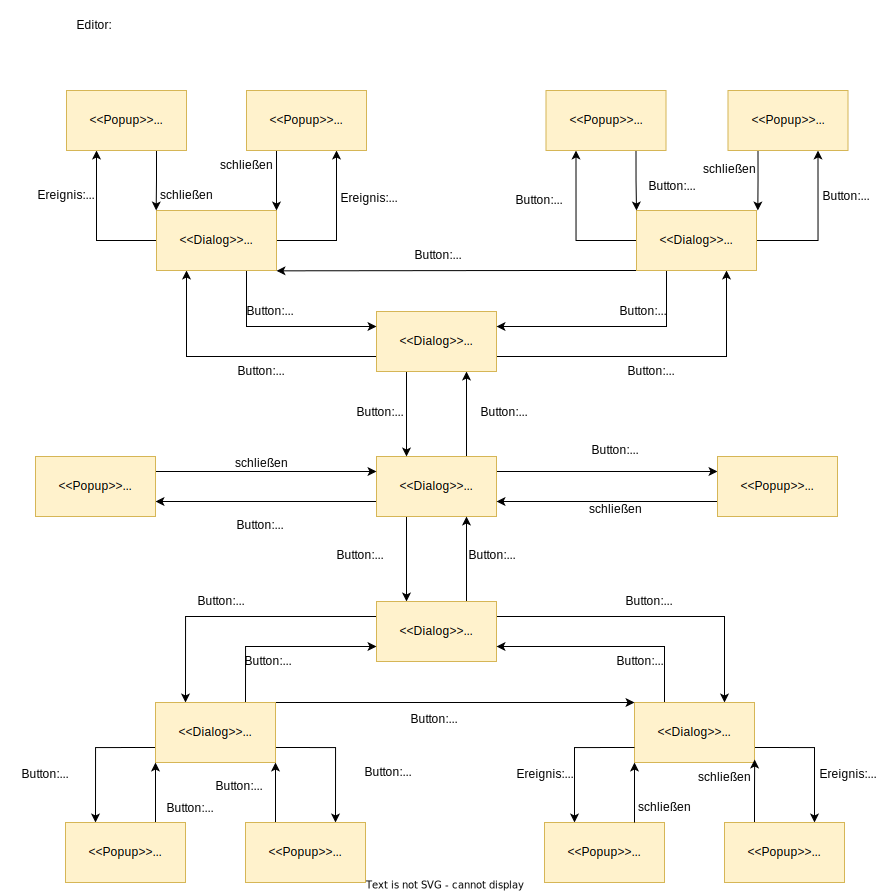
\includegraphics[width=\textwidth]{Editor.drawio.png}
        \caption{Editor}
    \end{figure}

    \subsubsection{Benutzer-Client}
Da das Spiel intuitiv und schön zu bedienen sein soll macht es Sinn hier als Schnittstelle eine GUI zu wählen.
Der Benutzer-Client dient größtenteils dem Spielen und benötigt deshalb auch eine Darstellung der aktuellen Spielstands, des Spielfelds, der Karten und der Spielerpositionen. Hierfür ist eine grafische Darstellung natürlich deutlich angenehmer und übersichtlicher.

    \begin{figure}[H]
        \centering
        \includegraphics[width=\textwidth] {Benutzer-Client.pdf}
        \caption{Benutzer-Client}
    \end{figure}

    
    
    \subsubsection{sonstige Dialogstrukturdiagramme}
    \begin{figure}[H]
        \centering
        \includegraphics[width=\textwidth]{VF.pdf}
        \caption{Verbindungsfehler}
    \end{figure}

    \begin{figure}[H]
        \centering
        \includegraphics[width=\textwidth] {PF.pdf}
        \caption{unbekanter Fehler}
    \end{figure}
    


    \section{Mocks-Up}

Mocks-Up sollen denn Eindruck geben, wie das System visuell aussehen soll. Folgende Abbildungen sind Start, Enter, Settings, Gameboard, Select Cards and Endcard.

     \begin{figure}[h]
        \centering
        \includegraphics[width=\textwidth] {Start.png}
        \caption{Start}
    \end{figure}

    \begin{figure}
        \centering
        \includegraphics[width=\textwidth] {Enter.png}
        \caption{Enter}
    \end{figure}

    \begin{figure}
    \centering
        \includegraphics[width=\textwidth] {Settings.png}
        \caption{Settings}
    \end{figure}

    \begin{figure}
        \centering
        \includegraphics[width=\textwidth]{Gameboard.png}
        \caption{Gameboard}
    \end{figure}

    \begin{figure}
        \centering
        \includegraphics[width=\textwidth] {SelectCard.png}
        \caption{Select Cards}
    \end{figure}

     \begin{figure}
        \centering
        \includegraphics[width=\textwidth]{Endcard.png}
        \caption{Endcard}
    \end{figure}

    
\end{document}
\end{document}